
\cleardoublepage


\chapter{Northeast Beam Port Modeling}


\section{Introduction}

% here, introduce the ideas present in chapter 3
This section contains a complete description of the neutronic modeling for the NEBP.
% before you measure it, it helps to have a model
It is often necessary, as in this case, to model a neutronic environment before attempting to measure it, as the modeling results can inform certain measurement methods and parameters.
The measurement systems used in later analyses required calculated response functions that incorporated the flux's angular dependence obtained from this modeling effort.
The final result from this section also provides the default spectrum to be used in the unfolding of the neutron spectrum after measurement.
% there were many problems encountered along the way that lengthened the process of obtaining the final results, most regarding computation time
Many problems were encountered during this analysis, often related to computational difficulty/time, that lengthened the process of obtaining the final results.
These problems, along with the applied solutions, are presented.
% first mcnp kcode, then sdef, then advantg, then finally the tally results
We begin with the NEBP model's KCODE implementation in MCNP, followed by a conversion to a steady-state problem, the application of variance reduction, and finally, the beam-aperture tally results.
% the steps here ultimately led to success in solving a difficult transport problem and could be used in other things like this.
The steps here ultimately led to success in solving a difficult transport problem and these steps taken can likely be applied to similar situations, such as other reactor beam transport problems or, more broadly speaking, any problem with severe collimation of an isotropic source.

% ------------------------------------------------------------------------------
\section{Addition of Northeast Beam Port}


\subsection{Existing Model}

% introduce the idea of the model
% talk about the effort
In the summer of 2017, a reactor modeling effort was initiated at KSU.
% why it started
The goal of the effort was to produce, from the ground up, a Python-based suite that would interpret geometric and material data related to KSU's TRIGA Mark II research reactor and produce input files for various transport codes.
% what has been produced so far
The model, though still currently under development, contains a majority of the features from the actual reactor, including any of those which would have a major neutronic impact.
There are 85 fuel elements, containing fresh fuel, that are able to be automatically discretized axially, radially, and azimuthally into up to 10,000 cells.
The four control rods are also included, and a user may specify their exact position to match that of in-core experiments.
The central thimble, grid plates, and source location are all also included in the core model, which is surrounded by a graphite reflector.
This model can be seen in \FIG{fig:existing} and can be used to create input files for different transport codes, such as MCNP \cite{goorley2012initial}.

% the existing reactor model
\begin{figure}
\centering
\subfloat[$yz$]{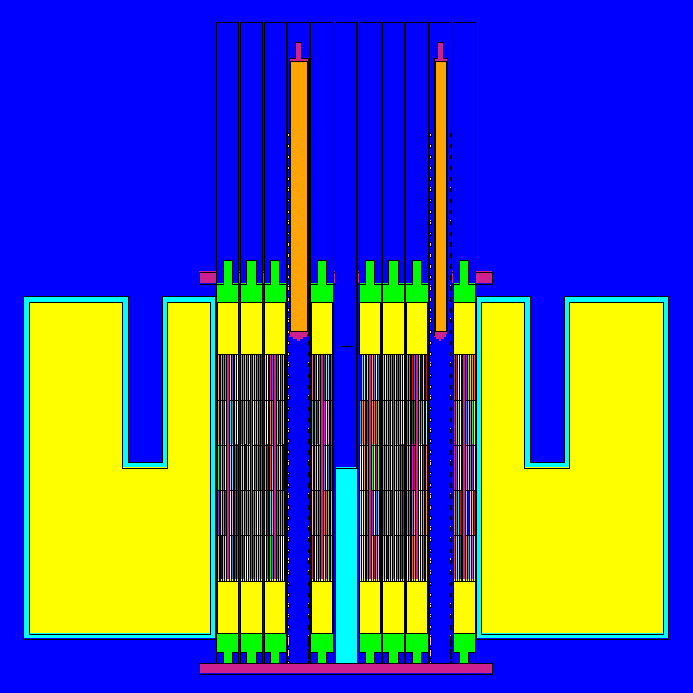
\includegraphics[height=3in]{tex/figures/existingyz.png}} 
\subfloat[$xy$]{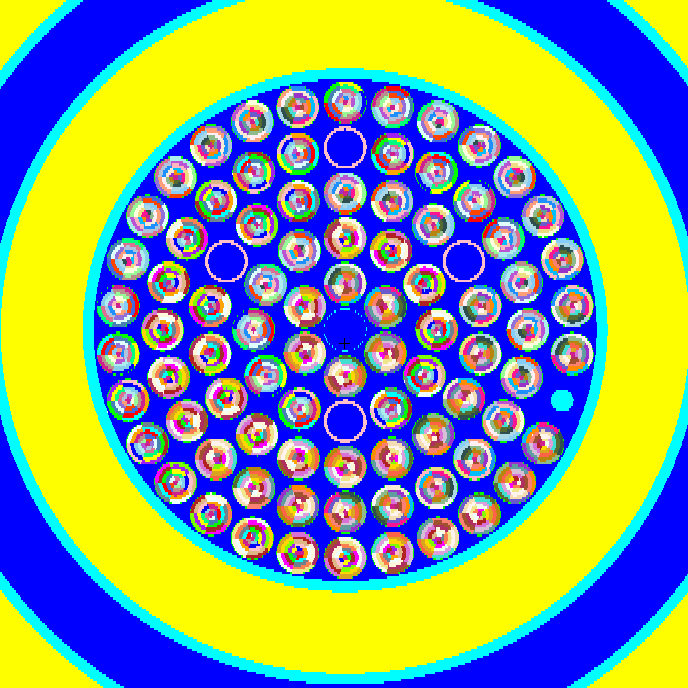
\includegraphics[height=3in]{tex/figures/existingxy.png}}
\caption[Old Reactor Model]{A $yz$ and $xy$ slice of the existing reactor model before the addition of the beam port.}
\label{fig:existing}
\end{figure}


\subsection{The Beam Port Geometry}

% introduce
Using this model as a starting point, the northeast beam port (NEBP) was then added.
% what is the beam port
The NEBP, also known as the penetrating beam port or the fast beam port, is in essence a large, collimating cavity in the reactor's structure that allows neutrons to stream from the core to the outside of the reactor.
% purpose
The primary purpose of this beam is to provide a monodirectional neutron source, the strength of which can be scaled easily via reactor control.
This beam can be used for detector calibrations and testing, neutron imaging, or sample irradiation for neutron activation analysis.
The NEBP is unique in the fact that it penetrates the graphite reflector providing, in theory, the hardest neutron spectrum of the four beam ports at KSU due to the absence of significant moderating material between the fuel and the beam port, as all other beam ports are located outside of the graphite reflector.

% isometric view of the solidworks model of the beam port
\begin{figure}[htb]
\centering
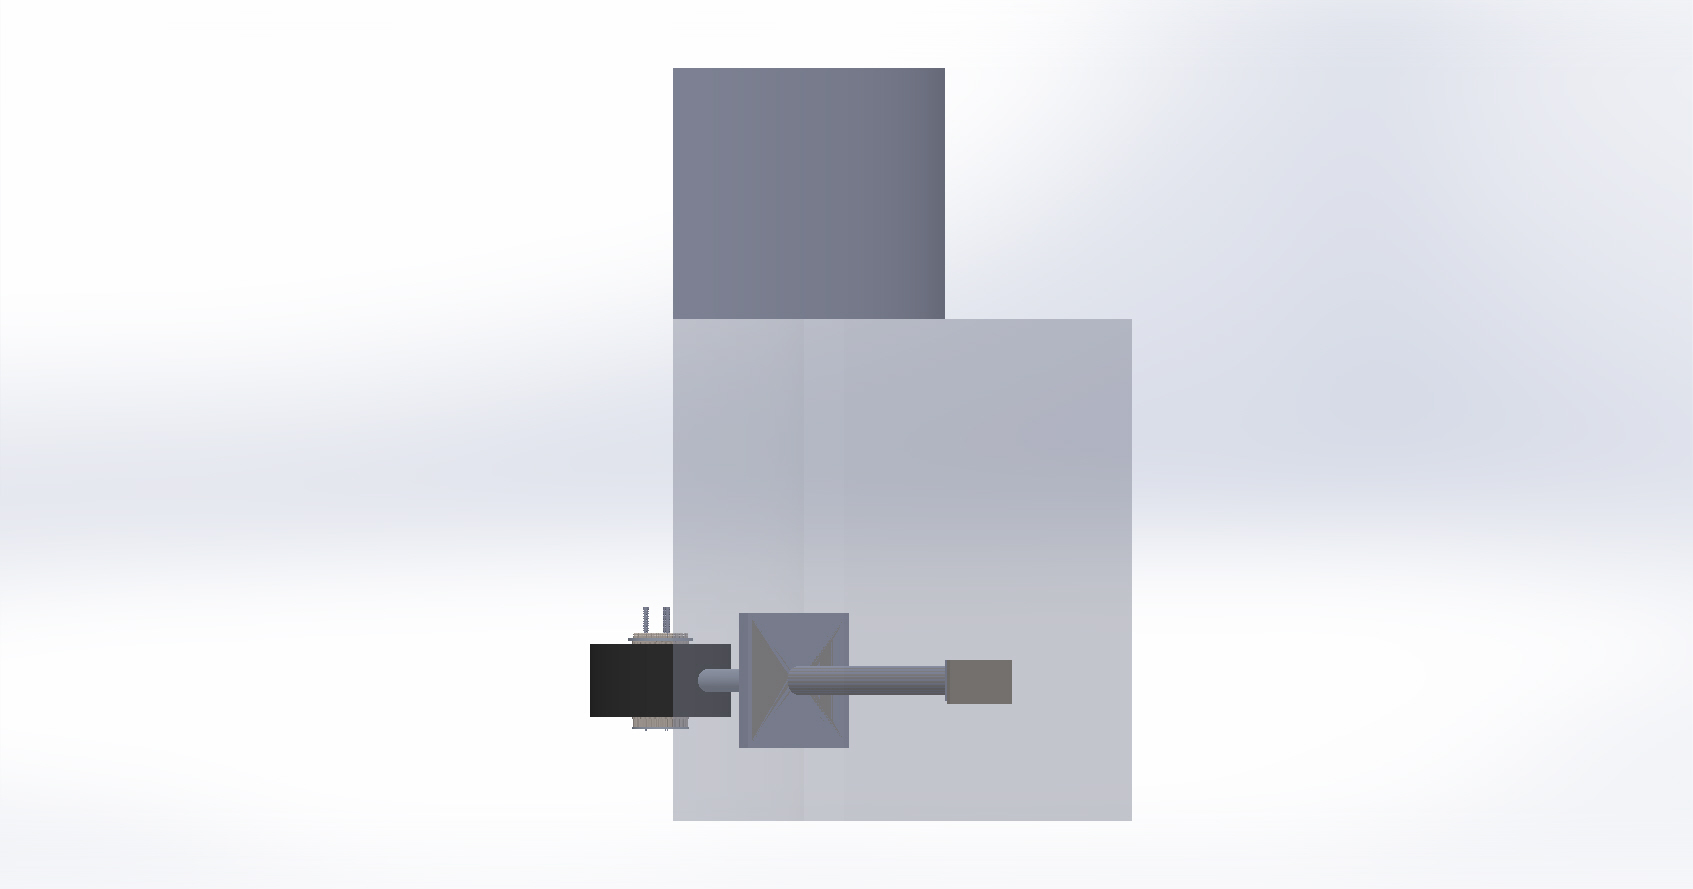
\includegraphics[height=3in]{tex/figures/solidworksangled.jpg}
\caption[Solidworks Angled NEBP]{An angled view of the NEBP with the reactor with a quarter section of the reactor structure.}
\label{fig:solidworksangled}
\end{figure}


The NEBP geometry is relatively simple.
% two sections 6 and 8 inch
It is comprised of two, six-foot, cylindrical segments; the inner and outer segments being 6 in and 8 in in diameter, respectively.
% coupled by shadow shield
A lead ``shadow shield" sits at the junction of these two sections to help reduce the gamma component of the outgoing particle stream.
The shadow shield is 4 ft x 4 ft and 4 in thick and contains a hole through the center, through which the outer portion of the NEBP's 6 in section extends.
% material
The walls of each section are made of 11/32" thick aluminum.
% wooden plugs but now empty
Originally, these sections contained removable wooden plugs that would block neutron streaming; however, water leaks in the port caused damage to these plugs, and, at present, they have been removed.

% collimator
A collimator is situated within the 8" section.
% who made it
This was designed by a KSU senior design team attempting to further constrain the neutron beam.
% describe design
The collimator is an aluminum tube of 0.75" ID and 1" OD.
An aluminum plate is affixed to this tube on the reactor side and contains a throughhole to maintain line of sight with the reactor core.
Borated polyethylene disks have been stacked around the tube to act as the primary absorption medium for collimating neutrons.
The borated polyethylene extends the entire distance of the collimator. 


\subsection{MCNP Implementation}

% mcnp with beamport geometry (zx)
\begin{figure}[htb]
\centering
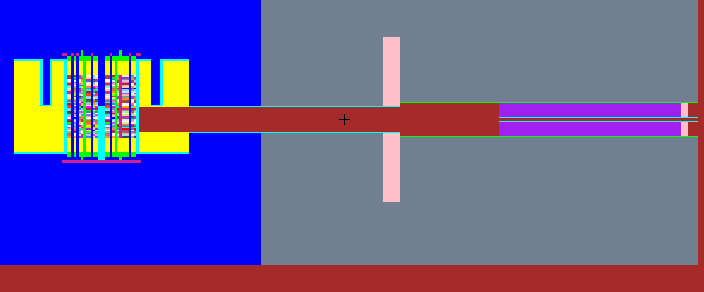
\includegraphics[height=2.5in]{tex/figures/mcnp_newxz.png}
\caption[MCNP NEBP $XZ$]{An $xz$ view of the NEBP in mcnp.}
\label{fig:mcnp_newxz}
\end{figure}

% the xy view of the nebp in mcnp
\begin{figure}[htb]
\centering
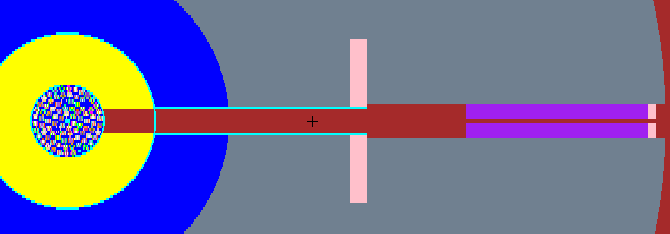
\includegraphics[width=1\textwidth]{tex/figures/mcnp_newxy.png}
\caption[MCNP NEBP $XY$]{An $xy$ view of the NEBP in mcnp.}
\label{fig:mcnp_newxy}
\end{figure}


% Write about the actual implementation
The NEBP itself consists primarily of cylinders and planes, so its implementation in the model was relatively straightforward.
The surrounding concrete structural region was modeled as a large cylindrical cell, with the assumption that the geometric intracies a great distance from the NEBP would have a minimal effect on the flux in the NEBP.
As described above, the NEBP, including both sections and the shadow shield, was added within this concrete region.
% hole in the graphite reflector
A penetration was added to the existing graphite reflector.
The reactor documentation was unclear about some specifics regarding this penetration, so it was assumed that it was not radially encased by any aluminum, but the aluminum surrounding the reflector was left intact to not let water in.
The materials used for the NEBP can be seen in \TAB{tab:nebp_materials}.
Material data in the model came from {\tt pyne} \cite{scopatz2012pyne}.


% table that contains the material data for the model
% density of steel 8.03

\begin{table}[h]\centering
\label{tab:nebp_materials}
\caption{Materials used in the NEBP model.}
\begin{tabular}{ r c l }
\toprule
\textbf{Material} & \textbf{Density} $g/cm^3$ & \textbf{Composition (Wgt. Fraction)} \\
\midrule
Aluminum & 2.7 & $^{27}$Al (1.000) \\
\midrule
Lead & 11.34 & $^{204}$Pb (0.0138)  $^{206}$Pb (0.2396) \\
        & & $^{207}$Pb (0.2207)  $^{208}$Pb (0.5259) \\
\midrule
Air & 0.001239 & $^{12}$C (0.0001)  $^{14}$N (0.7147) \\
        & & $^{16}$O (0.205)  $^{40}$Ar (0.0346) \\
\midrule
Borated Polyethylene & 0.95 & $^{1}$H (0.1253)  $^{2}$H (0.000028) \\
                       &  & $^{10}$B (0.0184)   $^{11}$B (0.0816) \\
                       &  & $^{12}$C (0.7657)   $^{13}$C (0.0090) \\
\midrule
Concrete & 2.4 &  $^{1}$H (0.0221) $^{2}$H (0.00000509) \\
& &         $^{12}$C (0.002458)  $^{13}$C (0.0000288) \\
& &           $^{16}$O (0.5741)  $^{17}$O (0.000232) \\
& &          $^{23}$Na (0.0152)   $^{24}$Mg (0.000988) \\
& &          $^{25}$Mg (0.00013)   $^{26}$Mg (0.000149) \\
& &          $^{27}$Al (0.01998)   $^{28}$Si (0.2802) \\
& &          $^{29}$Si (0.0147)  $^{30}$Si (0.010066) \\
& &          $^{39}$K (0.0093)   $^{40}$K (0.0000012) \\
& &          $^{41}$K (0.000709)  $^{40}$Ca (0.04157) \\
& &          $^{42}$Ca (0.00029)    $^{43}$Ca (0.00006223) \\
& &          $^{44}$Ca (0.00098)   $^{46}$Ca (0.00000197) \\
& &          $^{48}$Ca (0.00009622)    $^{54}$Fe (0.00036) \\
& &          $^{56}$Fe (0.00592)   $^{57}$Fe (0.000139) \\
& &          $^{58}$Fe (0.0000189) \\
\midrule
Steel & 8.03 & $^{12}$C (0.00039536233)  $^{13}$C (0.0000046336713) \\
& &            $^{28}$Si (0.0045932784) $^{29}$Si  (0.00024167903) \\
& &            $^{30}$Si  (0.00016499257) $^{31}$P  (0.0002299977) \\
& &            $^{32}$S  (0.00014207158)  $^{33}$S  (0.0000011567992) \\
& &            $^{34}$S  (0.0000067532956) $^{36}$S  (0.000000016825336) \\
& &            $^{50}$Cr  (0.007929925)   $^{52}$Cr  (0.1590272) \\
& &            $^{53}$Cr  (0.018379631)   $^{54}$Cr  (0.0046613454) \\
& &            $^{55}$Mn  (0.0099999)   $^{54}$Fe  (0.03961618) \\
& &            $^{56}$Fe  (0.64489415)   $^{57}$Fe  (0.015159803) \\
& &            $^{58}$Fe  (0.0020528512)  $^{58}$Ni  (0.062157351) \\
& &            $^{60}$Ni  (0.024767425)  $^{61}$Ni  (0.0010945963) \\
& &            $^{62}$Ni  (0.003547273)  $^{64}$Ni  (0.00093242912) \\
\bottomrule
\end{tabular}
\end{table}

\clearpage

% ------------------------------------------------------------------------------
\section{Fission Rate Tallying and Steady-State Source Generation}
\subsection{SDEF Generation}

% the goal is transport, so no kcode
The ultimate goal here is to obtain, via simulation, the flux departing from the beam port.
However, the existing model is setup only for KCODE problems.
The difficult nature of this transport problem, due to the low probability of a simulated particle streaming down the collimator and exiting the reactor, requires some form of variance reduction.
Because of an incompatibility between KCODE problems and the code ADVANTG (selected for variance reduction and used to generate weight windows), this problem must first be converted into an SDEF-type problem.
This conversion required the collection of spatially-dependent fission site data.
This ``fission map'' could provide the set of probability vectors to inform the source sampling in the steady-state problem.
This was done in the following way.
First, the fuel cells were discretized axially and radially.
It was decided to use 40 axial sections and 5 radial sections for each of the 85 fuel elements to create a total of 17,000 individual cells.
This resolution ensured that the details in the fission rate profiles were adequately captured.
Then a fission rate tally was created for these cells.
This was done using an F4 tally (flux averaged over a cell) with an FM (tally multiplier) card which would multiply the flux by the total fission cross section for the fresh fuel material.
With these tallys in place, the KCODE problem was then run for a total of 4,400 cycles where the first 10 were discarded and each cycle consisted of 100,000 particles.
This guaranteed the statistics for the tallies had properly converged.

After running this problem, a python script was used to parse the output and generate an SDEF source to be used in the next step; this card is:

\begin{center}
{\tt SDEF ERG=D1 RAD=D2  AXS=0 0 1  POS=D3  EXT=FPOS=D4}
\end{center}

\noindent
The {\tt ERG} (energy) distribution used for the source was MCNP's built-in Watt spectrum, indicated by a {\tt -3} on the source probability card.
The source's spatial distribution is a series of cylinders co-located with the respective fuel elements within the core.
The {\tt POS} (position) variable contained the center points of each of the fuel elements, whose probability of sampling is proportional to their integrated fission rate.
The {\tt EXT} (extent) variable means length of the cylinder, in this case the length of the fuel meat, and refers to a series of distributions dependent on the {\tt POS} of the fuel.
Because base MCNP does not easily allow for nested dependent distributions, the {\tt RAD} (radial) distribution was considered an independent variable, and the distribution used was the normalized, averaged radial fission rate across each fuel element.

\subsection{Fission Tally Results}

% coremap
\begin{figure}[htb]
\centering
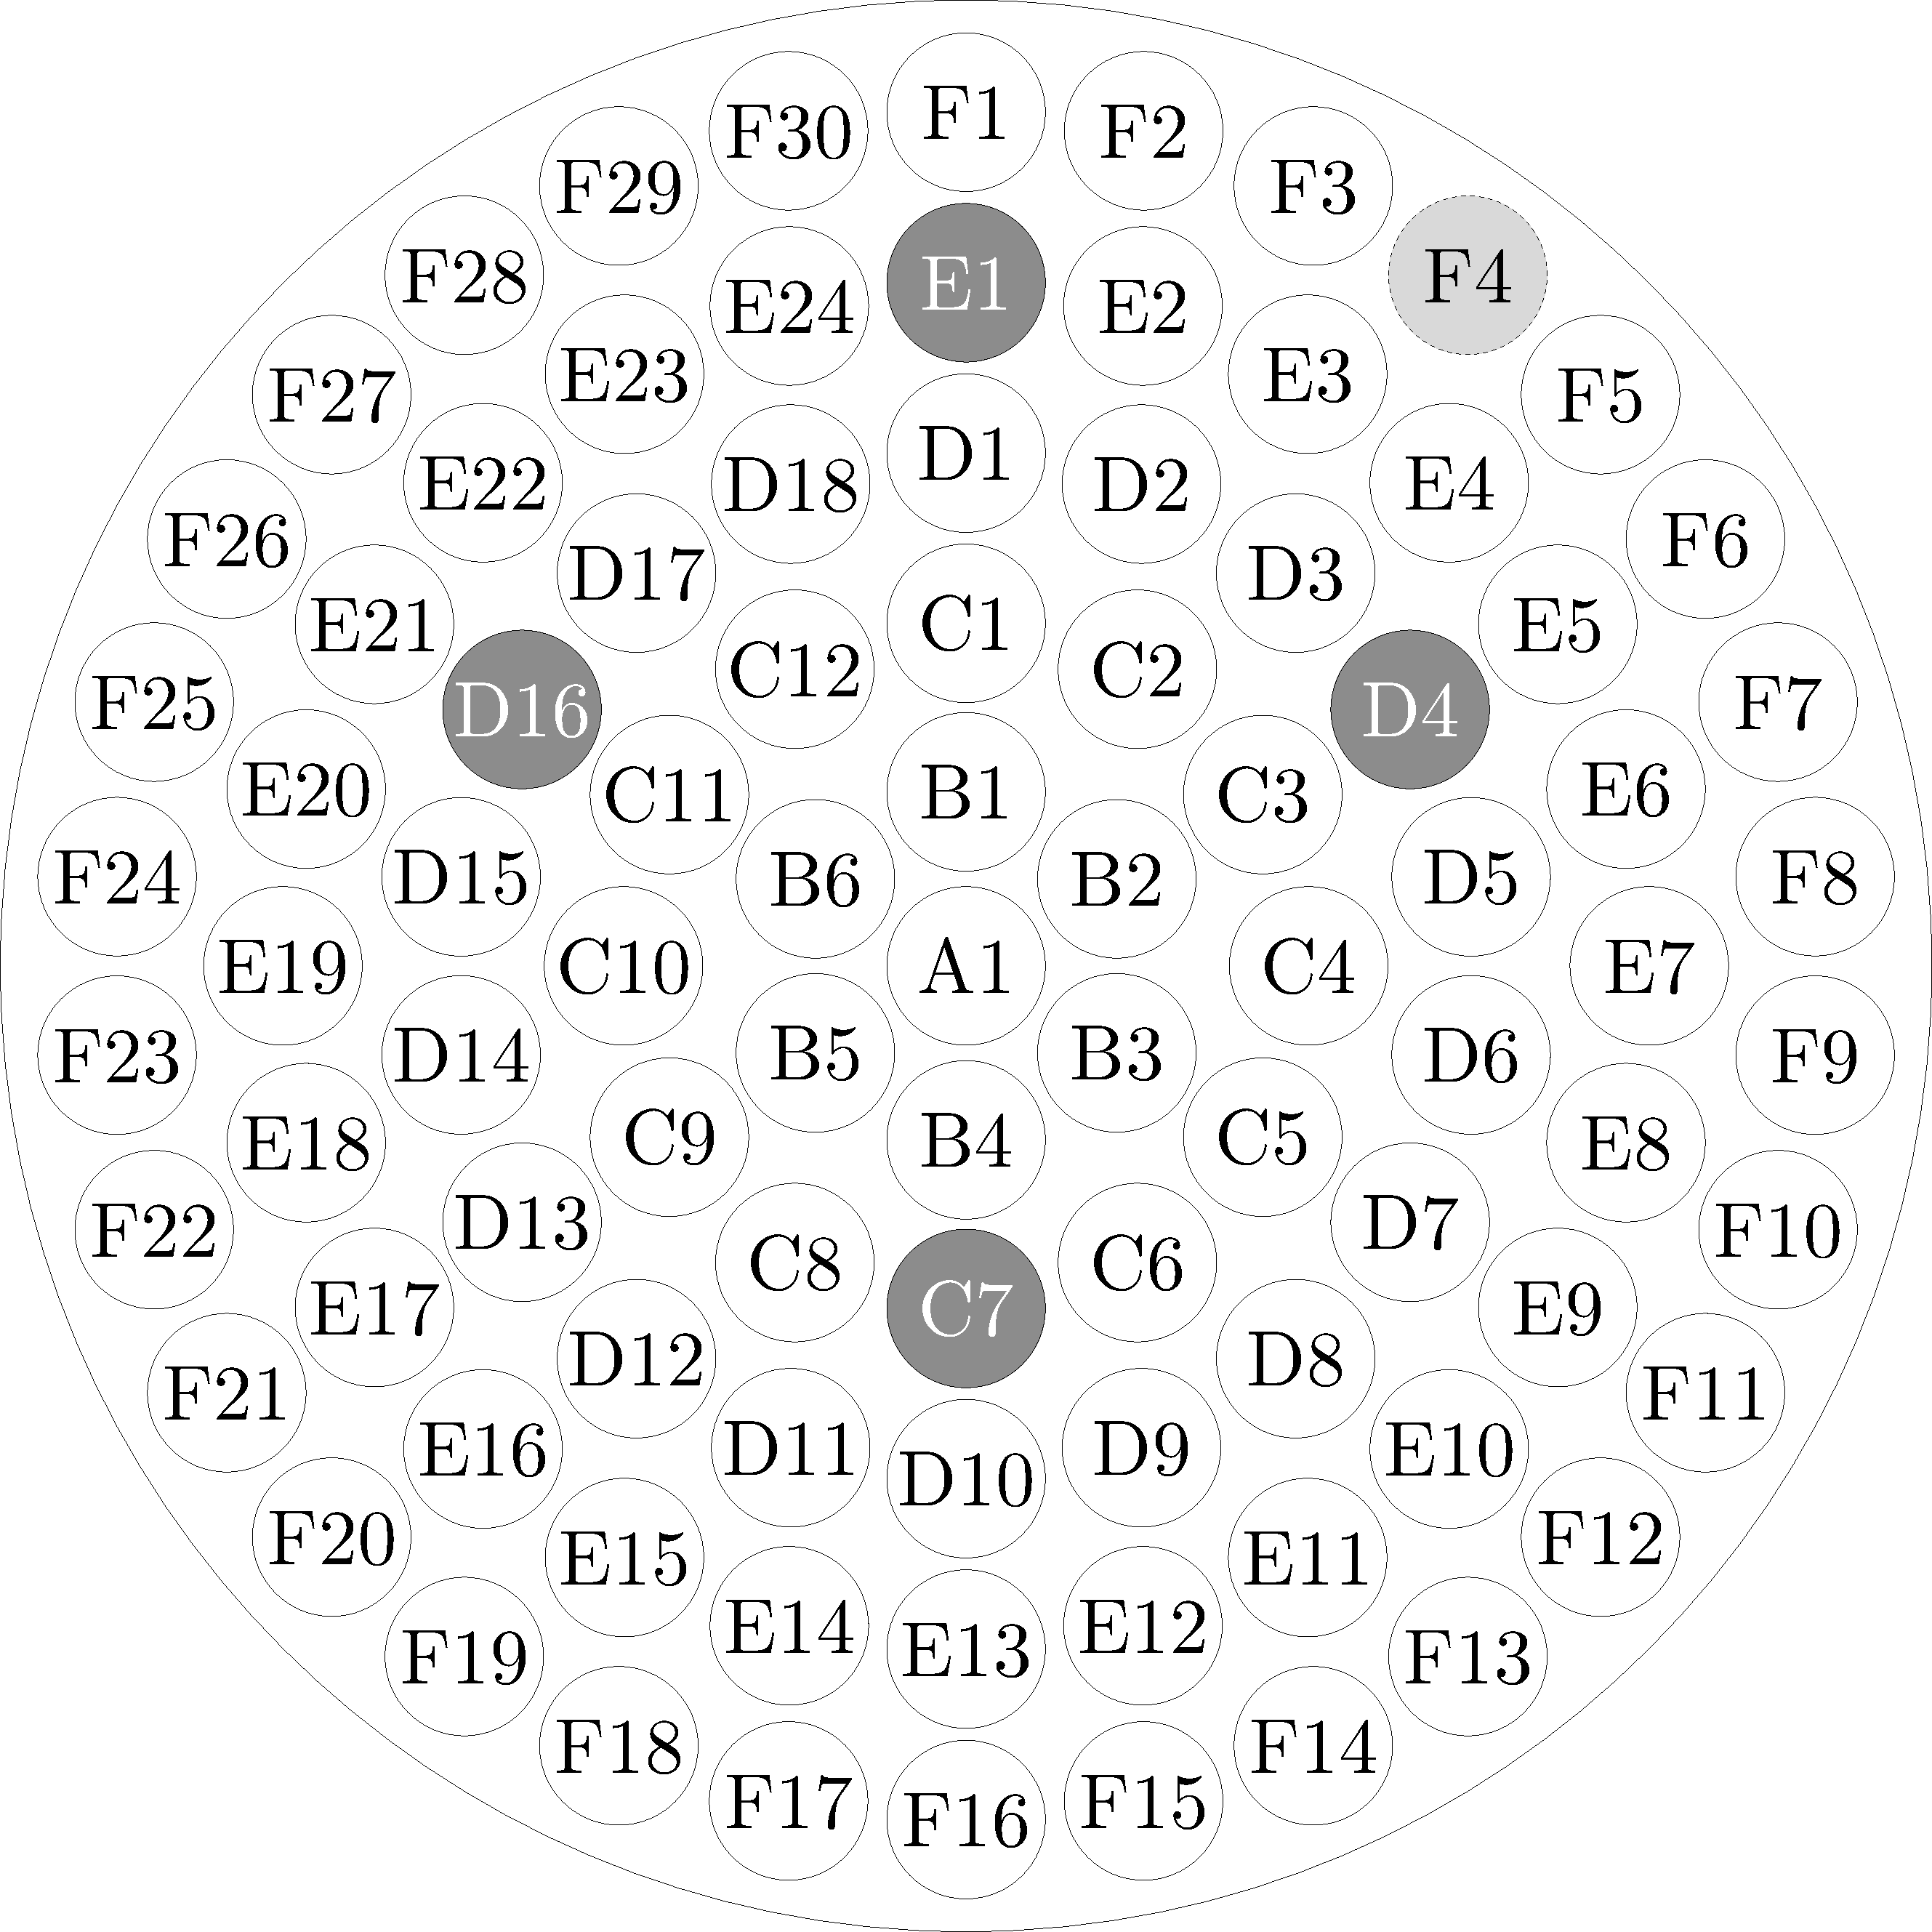
\includegraphics[height=4in]{tex/figures/coremap.pdf}
\caption[Core Map]{A map of the named elements in the core.}
\label{fig:coremap}
\end{figure}

For reference, a map of the core is provided in \FIG{fig:coremap}.
Along with the source, several plots were made of this fission rate data.

% the fission rates tallied inside a fuel element
\begin{figure}[htb]
\centering
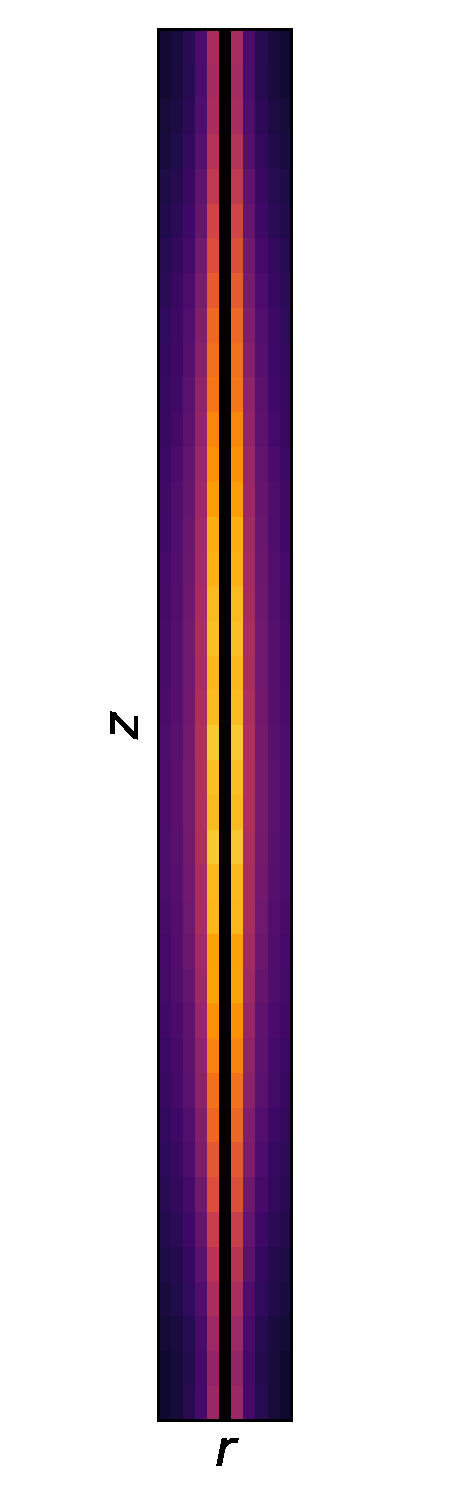
\includegraphics[height=4in]{tex/figures/rr_dist_B1.pdf}
\caption[Fission Rate Dist. B1]{The fission rate distribution within the element B1.}
\label{fig:rr_dist_b1}
\end{figure}

% talk about the B1 element plot
The heatmap in \FIG{fig:rr_dist_b1} demonstrates how the fissions are distributed within a typical fuel element.
Because there was no azimuthal discretization in the tallies, the values here are rotationally symmetric.
Although it is hard to draw any quantitative conclusions from this image, it is useful for visualizing fission rates within an element.
The fission rate appears to be a maximum at the center of the rod, both axially and radially.

% the radial reaction rate density within the B ring
\begin{figure}[htb]
\centering
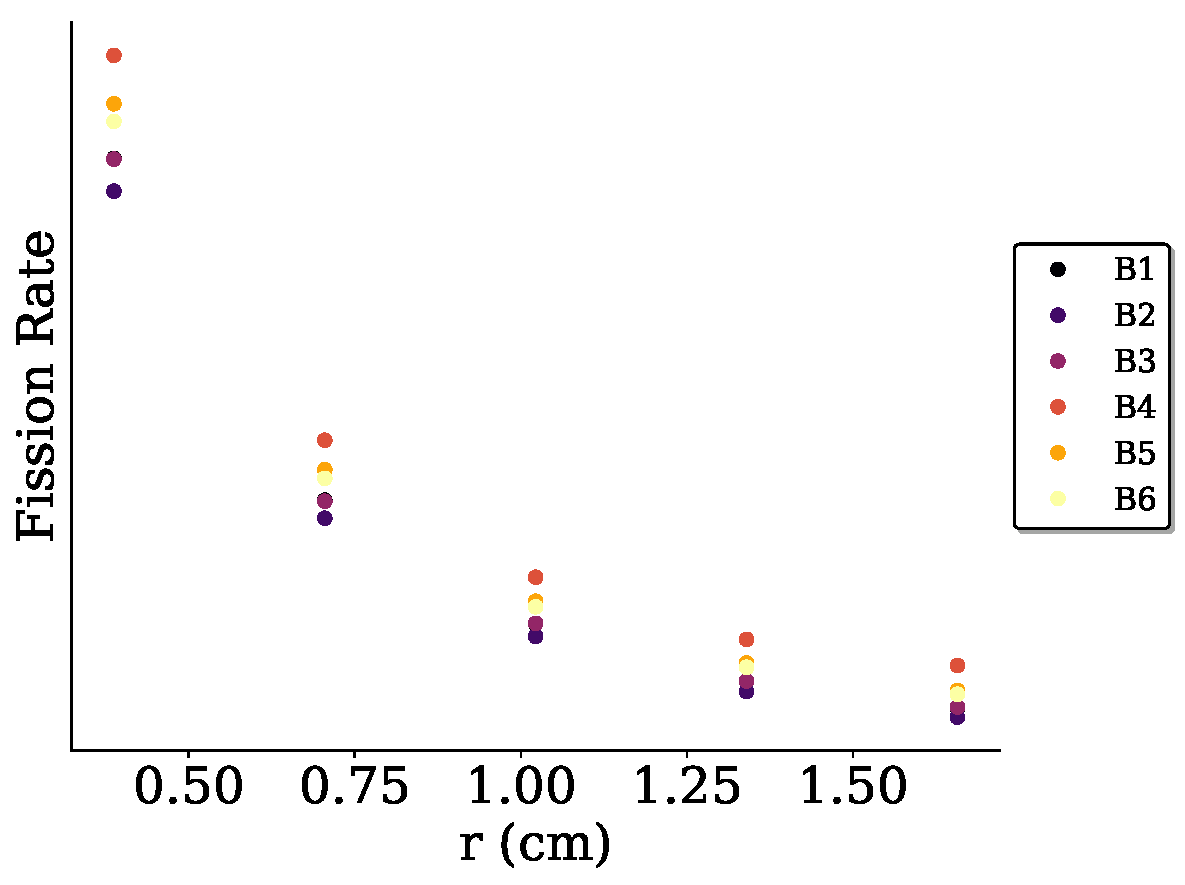
\includegraphics[height=4in]{tex/figures/radial_rr_density_B.pdf}
\caption[Radial Fission Rate Density B]{The radial fission rate within the B ring.}
\label{fig:radial_rr_density_B}
\end{figure}

In \FIG{fig:radial_rr_density_B}, one can see the radial behavior of the fission rates within ring B.
Although the curves here are different, they differ primarily in magnitude and not shape.
The other rings not pictured here all show similar behavior.
The fission rate density is highest towards the center of the rod and lowest in the outermost region.

% the axial reaction rate densities
\begin{figure}[htb]
\centering
\subfloat[B Ring]{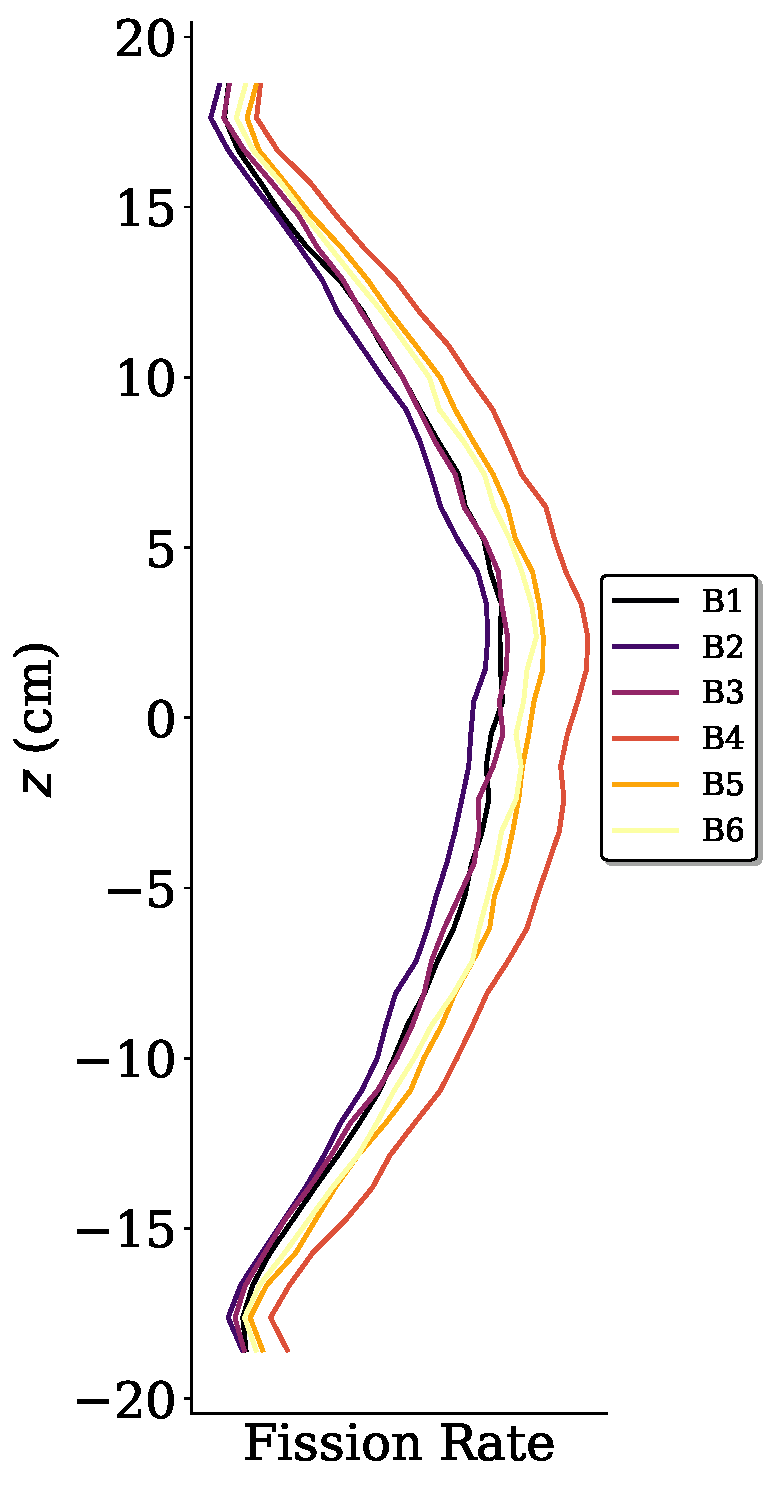
\includegraphics[height = 4in]{tex/figures/axial_rr_density_B.pdf}} 
\subfloat[C Ring]{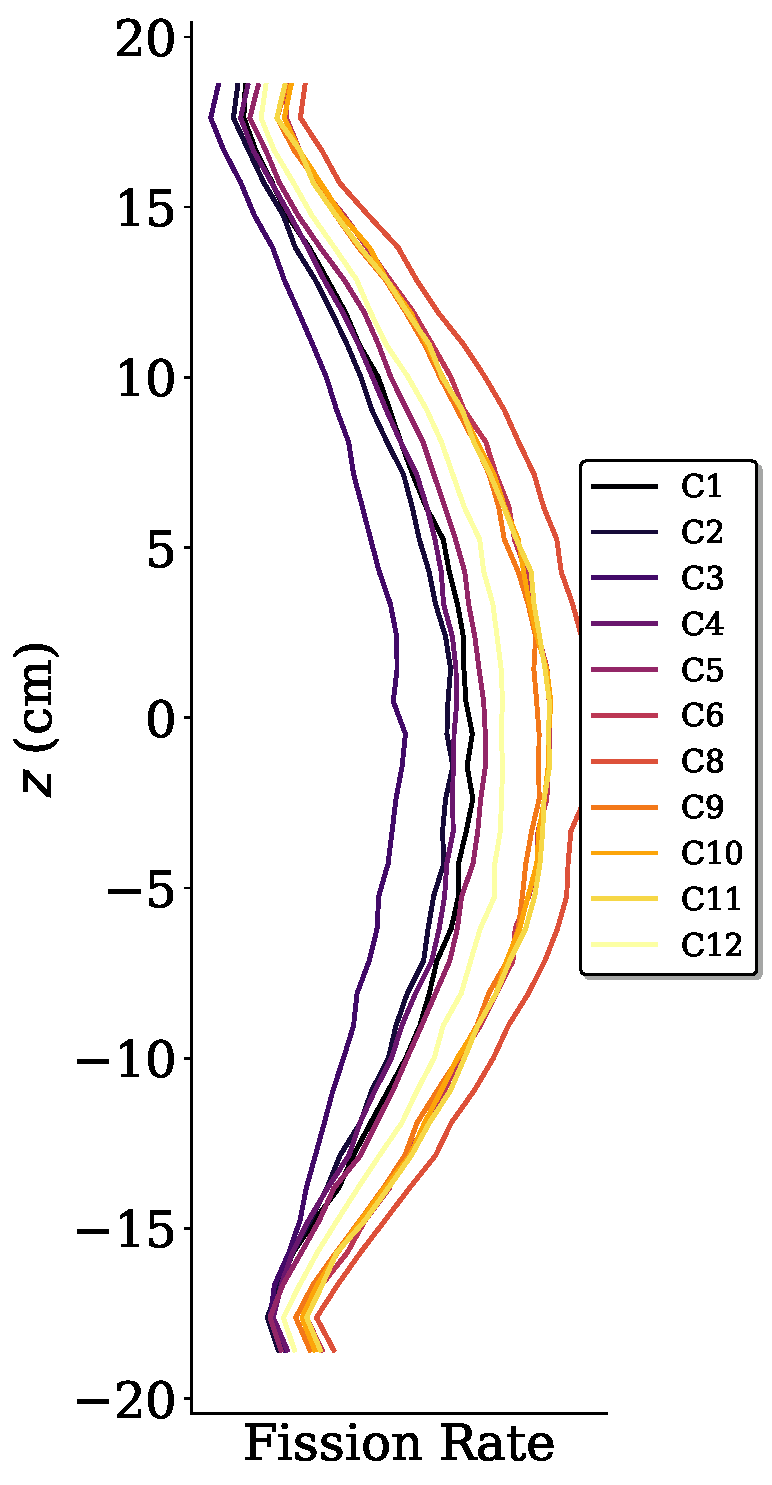
\includegraphics[height = 4in]{tex/figures/axial_rr_density_C.pdf}}
\subfloat[D Ring]{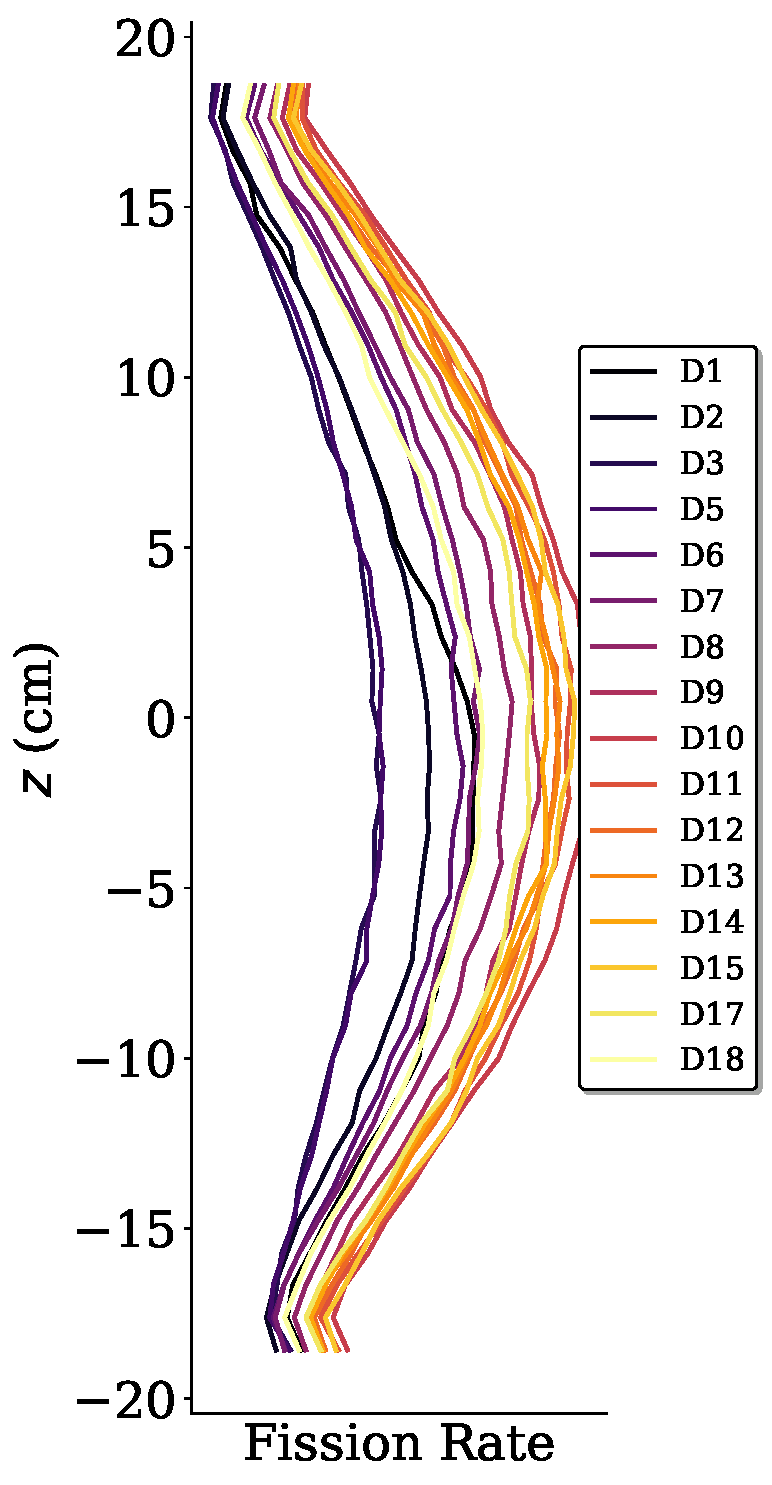
\includegraphics[height = 4in]{tex/figures/axial_rr_density_D.pdf}}\\
\subfloat[E Ring]{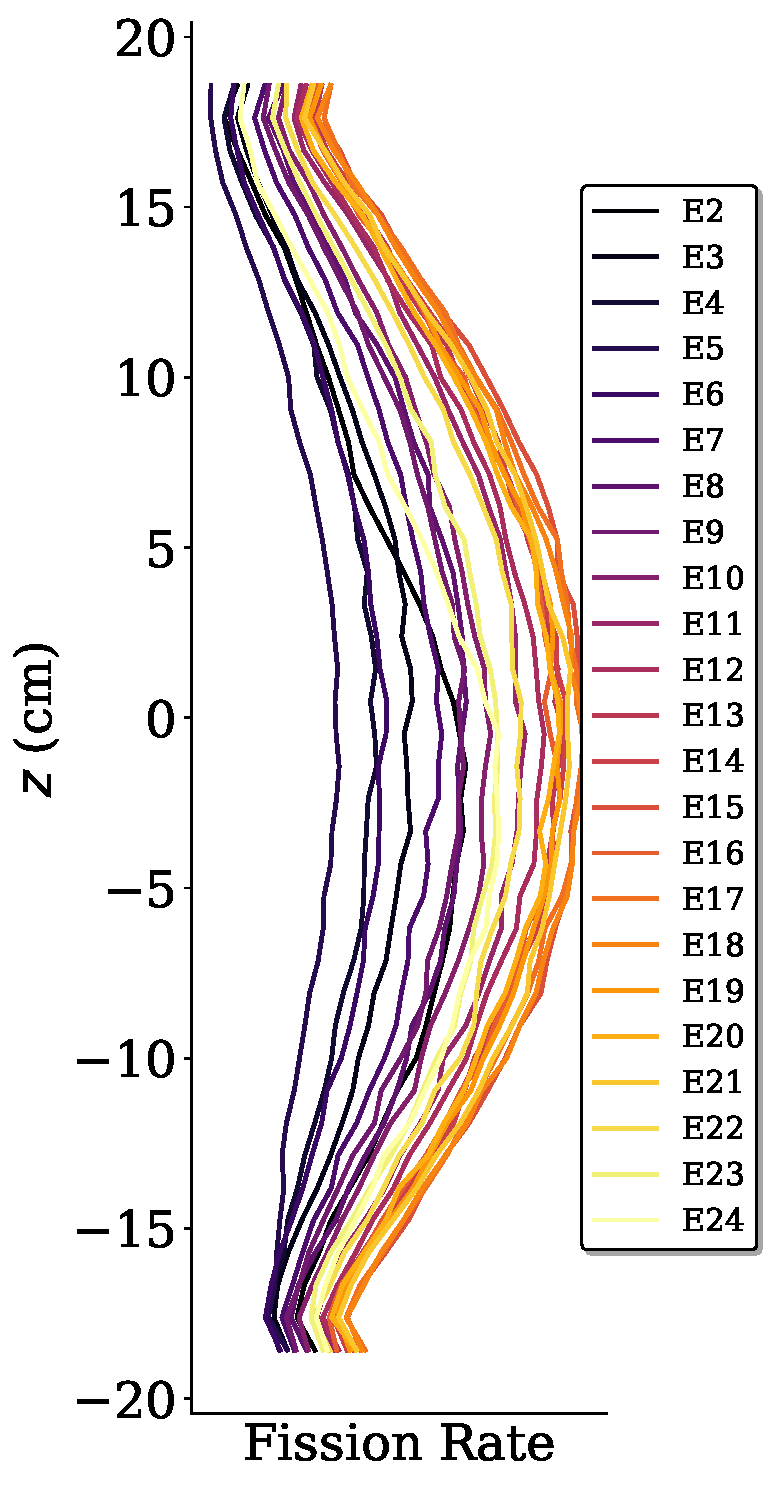
\includegraphics[height = 4in]{tex/figures/axial_rr_density_E.pdf}} 
\subfloat[F Ring]{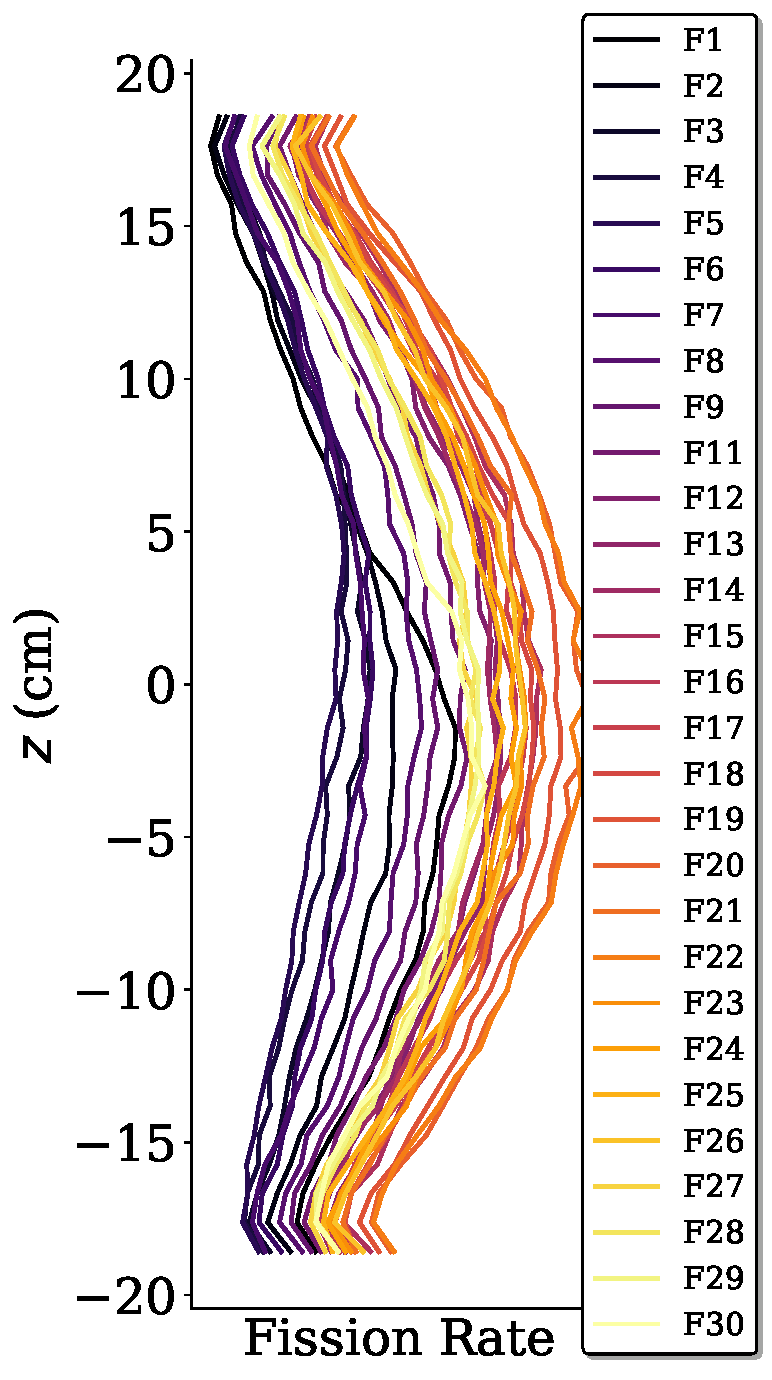
\includegraphics[height = 4in]{tex/figures/axial_rr_density_F.pdf}} 
\caption[Axial Fission Rates]{The axial fission rates within each ring of the core.}
\label{fig:axial_rr_density}
\end{figure}

\clearpage

\FIGURE{fig:axial_rr_density} shows the axial fission rate densities within each ring of the core.
Each of these rings shows a cosine-like distribution with a slight upturn at each extrema.
Neutron flux within a {\it roughly} cylindrical geometry, like a reactor core, will {\it roughly} exhibit a cosine shape, which causes a similar shape for the fission distribution.
The upturn is caused by the graphite on each end of the fuel elements which reflects neutrons back towards the rod.
There are two rings in particular that show additional behavior outside of these two phemonena.
The first is the depression within the B ring below 0 cm.
This is caused by the central thimble, which currently occupies the A1 location.
Moderating water which would normally occupy that location is replaced by this thimble which is currently modeled as an aluminum rod that extends halfway up the core.
This lack of neutron moderation means lower thermal flux in that region and results in the depression.

The second is the depressed fission rate within the lower region of F1-F9.
This is caused by the addition of the NEBP.
Recall, the beam port includes a penetration within the graphite reflector. 
This penetration is situated 8.3 cm below the z axis.
This lack of reflection means more neutrons will stream out of the core within that region, thus lowering the local flux and fission rate.
This effect can be seen to a degree within the E ring, but it is much less pronounced.

\clearpage

% the integrated fission rates for each ring
\begin{figure}[htb]
\centering
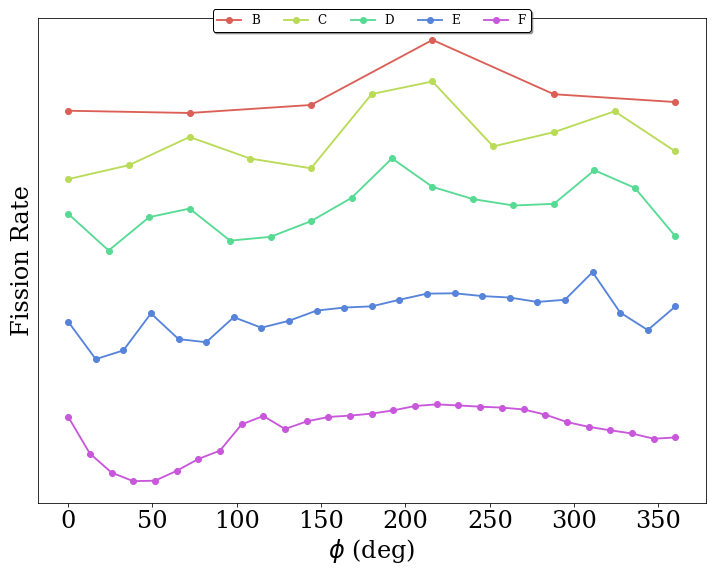
\includegraphics[height=5in]{tex/figures/totals_azi.png}
\caption[Whole Core Azimuthal Fission Rate Density]{The fission rate density for each element in the core as a function of core position.}
\label{fig:totals_azi}
\end{figure}

By studying \FIG{fig:totals_azi}, one can again see the effect the NEBP has on the F ring's fission rates.
This depression is seen when sweeping past the NEBP from around 12$^{\circ}$-75$^{\circ}$.
Other peaks and vallys seen in the figure are likely the cause of control rod, central thimble, and source placement.


% ------------------------------------------------------------------------------------------------------------------
\section{Application of ADVANTG}

% okay, we've got an SDEF problem, what kind of tallies would we like?
After obtaining the fission rate tallies and creating an appropriate SDEF card, the MCNP problem formulation is now only missing a final tally.
The tallies are setup here to capture the maximum detail and understanding of what is happening at the outer aperture of the NEBP.
First, the outer face of the NEBP is used in a surface tally (F2) to find the fluence departing.
This tally was divided spatially using different concentric cylinders, providing information on seven regions of the NEBP as shown in \FIG{fig:region_diagram}.
The first three are all equivalent-area tallies within the collimator itself.
This will provide an understanding of the radial distribution with the main beam.
The fourth segment was the exterior face of the aluminum collimator.
Then, the last three were equivalent area tallies within the borated polyethylene collimator.
This would give an idea for the quantity of neutrons that managed to escape the main beam but still contribute to detectors, dose, etc., outside of the beam.

% tally regions
\begin{figure}[htb]
\centering
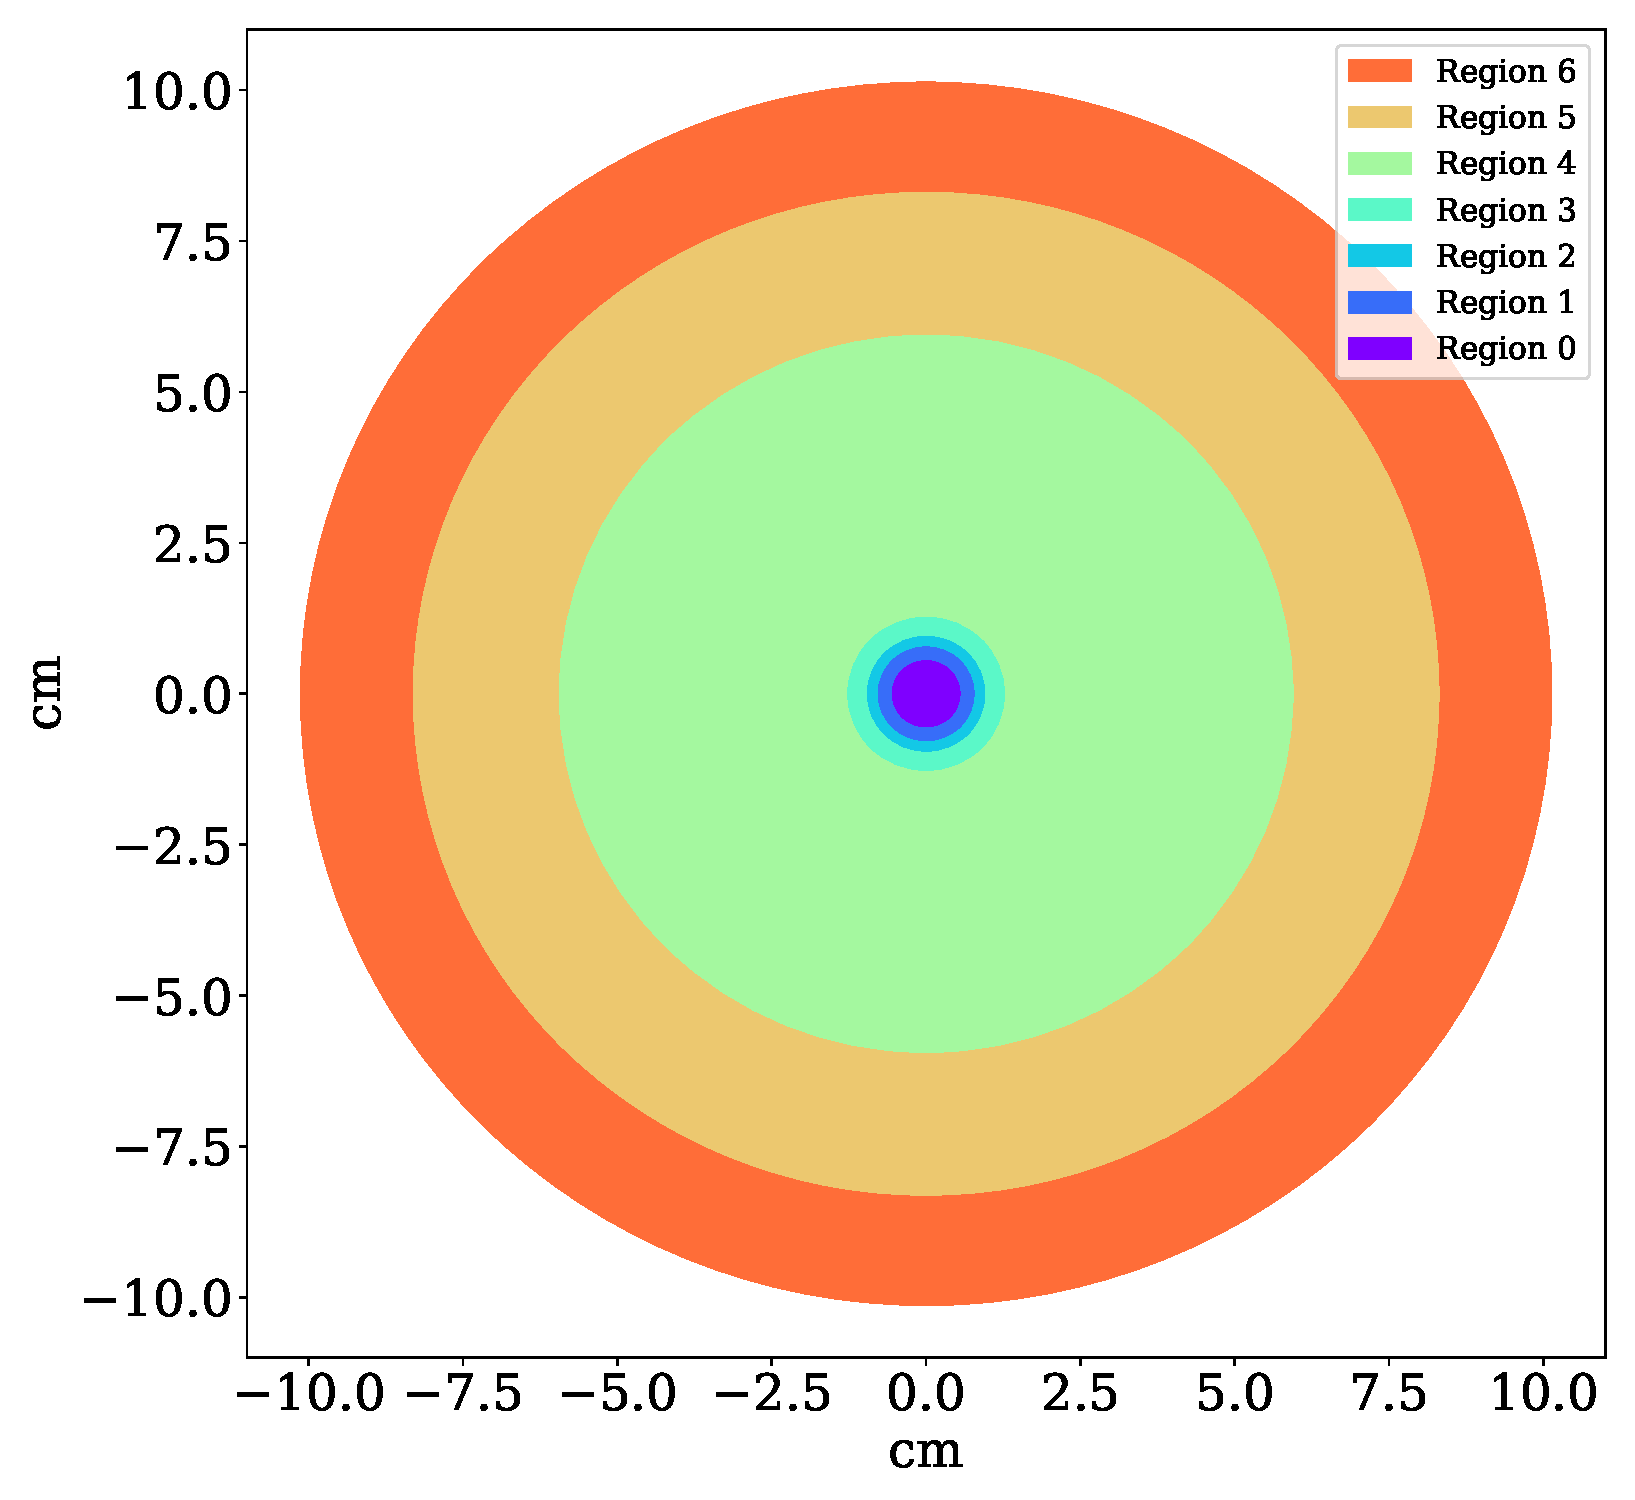
\includegraphics[height=5in]{tex/figures/region_diagram.pdf}
\caption[Tally Region Diagram]{The radial regions used for tallying.}
\label{fig:region_diagram}
\end{figure}

% we've also got them divided into cosine and energy
Then, both angular and spectral groupings were used to bin each of these regions.
For the angle, a custom, fine, 109-group structure was used.
The first 20 bins were tenth degree increments between 0$^{\circ}$ and 2$^{\circ}$, where 0$^{\circ}$ refers to a partition edge on the beam's main axis.
Following that, a resolution of one degree increments were used between 2$^{\circ}$ and 90$^{\circ}$
All of the backward fluence was captured by one bin between 90$^{\circ}$ and 180$^{\circ}$.

For the energy structure, the scale252 group structure was used.
This medium-resolution structure was selected because of the trade off between wanting to capture finer spectral details and the run-time to resolve statistics.

% great, can we run this?
With the tally now in place, MCNP was run, first without any variance reduction (VR).
Unsurprisingly, only a handful of the several million simulated particles survived to the end of the NEBP and were captured by the tally.
It became quickly apparent that this problem needed of some form of VR to be able to achieve decent tally results in any reasonable amount of time.

% let's pick advantg.
For this application, the code ADVANTG was select to provide the VR needed to do the transport.
% but what is advantg?
ADVANTG, the AutomateD VAriaNce reducTion Generator, generates weight window parameters for a fixed-source, continuous-energy MCNP problem \cite{mosher2013advantg}.
This is accomplished by solving the 3-D discrete ordinates neutron (or photon or coupled neutron-photon) transport problem using the Denovo package.
The adjoint solution obtained in this way is used to generate the weight window mesh to be used in the MCNP problem.
ADVANTG also creates biasing parameters for the source.
Both the weight windows and biasing parameters work together to provide a significant reduction in computational time for obtaining accurate tally results on difficult transport problems.
% then i'll explain why it's useful for our problem
In the case of the NEBP, the large source-to-tally distance, small tally solid angle, and large amount of present moderating and absorbing materials present a challenging transport problem, but one that ADVANTG can prove extremely useful to when applied.

% how did i apply it to our problem
However, there were first a few issues that needed to be addressed with the formulation of the transport problem before ADVANTG could be used effectively.
% first, we rotated the model
Recall that the NEBP aligns 50$^{\circ}$ azimuthally from the main $x$-axis.
Denovo \cite{evans2010denovo} solves problems on a 3-D fixed mesh, meaning that capturing the details of the NEBP will be counterintuitive, as the axis of the beam does not directly lie along one of the axes.
In addition to this, the full transport problem requires a large amount of memory to solve, which became a limiting factor when selecting ADVANTG parameters.
Because of these issues, the model needed to be rotated so that way the beam could lie on axis and the mesh resolution could be altered in a way that fully captured the effects of the beam and collimator while not wasting memory solving for fluxes in the structural material outside of the beam.
Alterations were then made to the input-generating python scripts to allow the user to rotate the entire model by altering a single parameter.
The model was then rotated 50$^{\circ}$ clockwise so the NEBP lied on the positive $x$-axis.
The KCODE problem was rerun to verify the rotated model still produced the same fission rates and that no biases were introduced.
The results from this verification did match the original fission-rate tallies.


% this contains all of the advantg parameters
\begin{table}[h]\centering
\label{tab:advantg_params}
\caption{Input parameters used for ADVANTG.}
\begin{tabular}{ r | l }
\toprule
model                     &   mcnp\\
method                    &   cadis\\
outputs                   &   mcnp\\
mcnp\_input               &   ksun.inp\\
mcnp\_tallies             &   11\\
mesh\_refinement          &   mcnp\\
mesh\_x                   &   -55 -22 22 184 368\\
mesh\_y                   &   -55 -22 -12 -2 2 12 22 55\\
mesh\_z                   &   -35 -16 -11 -5 0 35\\
mesh\_x\_ints             &   17 25 25 25\\
mesh\_y\_ints             &   75 14 17 22 17 14 17\\
mesh\_z\_ints             &   17 14 35 14 17\\
anisn\_library            &   bplus\\
denovo\_pn\_order         &   4\\
denovo\_quad\_num\_azi    &   15\\
denovo\_quad\_num\_polar  &   12\\
denovo\_x\_blocks         &   8\\
denovo\_y\_blocks         &   8\\
denovo\_z\_blocks         &   1\\
\end{tabular}
\end{table}

% then here, i'll just talk about all of the advantg parameters and why they were used
ADVANTG was then run with the NEBP problem.
The parameters selected are shown in \TAB{tab:advantg_params}.
% basically, everything comes down to runtime, memory, and FOM
Several of the parameters are self-explanatory, but the non-intuitive ones will be discussed here.
First, {\tt cadis} refers to the method used to solve the transport problem.
{\tt mesh\_x}, etc. refer to the major planes where the resolution of the mesh changes and {mesh\_x\_ints}, etc. refers to the number of elements between two planes in the mesh.
This mesh was selected to focus on the core and NEBP, so the region surrounding the beam is high resolution and the regions outside of the core and beam are low resolution.
The {\tt bplus} library was selected because it contained all of the materials used in the model and had a relatively large number of groups (47).
The degree of anisotropy modeled is adjusted by the {\tt denovo\_pn\_order}, which was selected to be 4.
A higher order in this case would increase the runtime, but not necessarily produce a more accurate solution for this particular problem.
The parameters, {\tt denovo\_quad\_num\_azi} and {\tt denovo\_quad\_num\_polar} refer to the number of angles used by the problem.
Because the problem has a high angular dependence (a beam of neutrons streaming down a long collimator), these were selected to be higher than the defaults.
Increasing this parameter also helped to reduce ray effects present within the solution.
Finally, {\tt denovo\_x\_blocks}, etc. refer to the parallelization scheme.
The computer used for this calculation had 64 cores available, so these values 8, 8, and 1 all multiply to that value.
% so i ran it, that gave me a wwinp file that was how many MB?
Using these parameters, ADVANTG was run and biasing parameters and a weight window input file was produced.

% denovo solutions
\begin{figure}[htb]
\centering
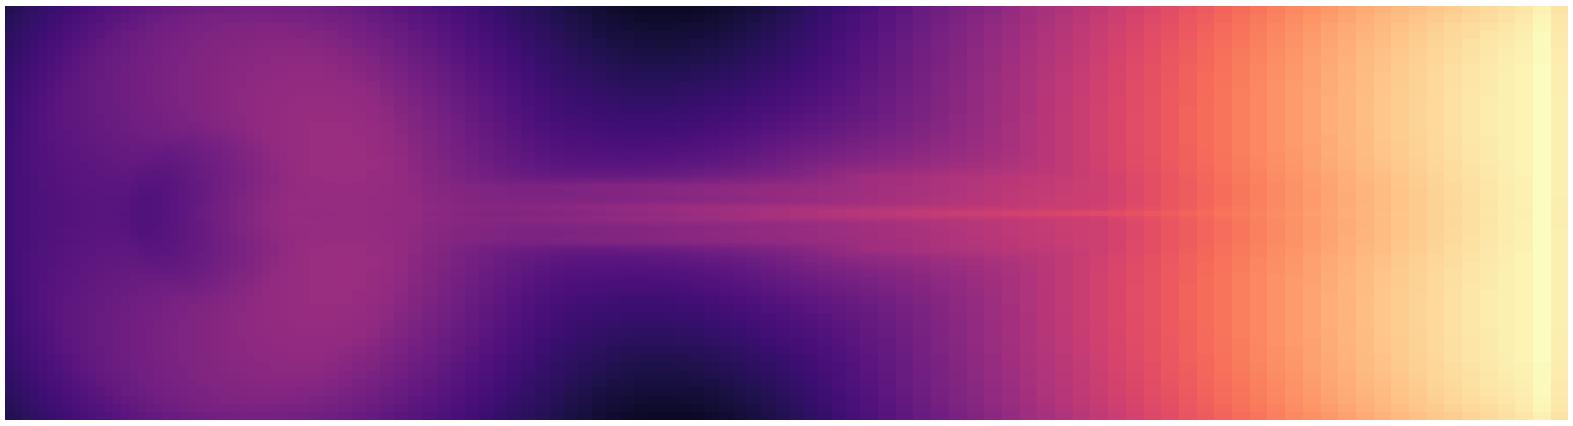
\includegraphics[width=0.8\textwidth]{tex/figures/advantgxy.png} 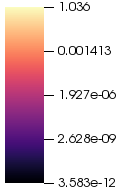
\includegraphics[width=0.14\textwidth]{tex/figures/advantg_legend.png}\\
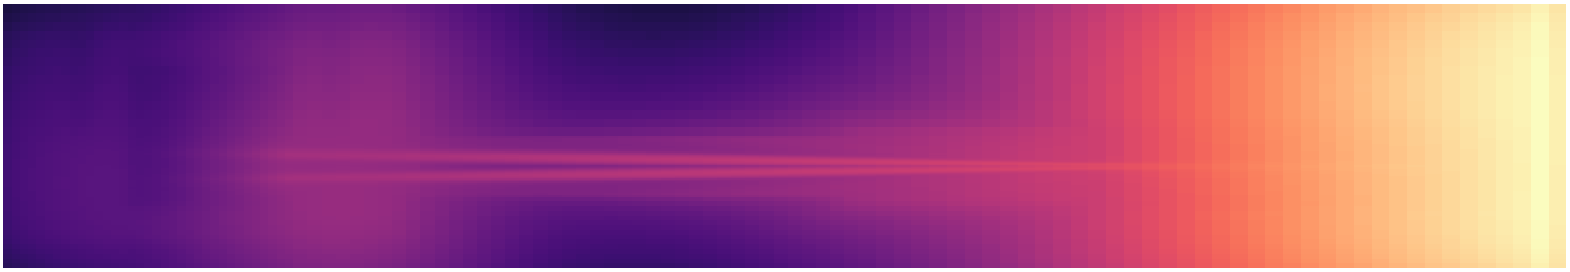
\includegraphics[width=\textwidth]{tex/figures/advantgxz.png}\\
\caption[ADVANTG Solution]{XY (top) and XZ (bottom) slices of the adjoint solution for group 6 (4.9659 - 6.0653 MeV) produced from ADVANTG. Units here are considered arbitrary as the weight window values produced from this solution will be normalized in the MCNP problem.}
\label{fig:advantg}
\end{figure}


% discuss the adjoint solution here
As an example, the adjoint flux solution for group 6 (4.9659 - 6.0653 MeV) can be seen in \FIG{fig:advantg}.
This solution allows us to see how the weight windows will be defined.
Regions with a high value have high "importance," i.e., neutrons in these regions are more likely to contribute to the response of interest.  As a particle moves from a region of low importance to one of higher importance, it is split into two or more identical particles of reduced weight such that the total weight is preserved.  This splitting process leads to a greater number of particles reaching the detector and, hence, lower uncertainties. 
The geometry of the core and beam are roughly apparent in the figure.
The side of the core closest to the beam is weighted higher than the side furthest, since neutrons born there are most likely to make it to the tally.
The highest values occur closest to the tally to ensure much splitting, and therefore, more particles tracked in the region of the tally.
In the reverse direction, some particles are killed ("rouletted"), while others are kept alive with increased weight, again, so that the total weight, on the average, is preserved. With this game of splitting and rouletting, the overall computational effort of moving particles is focused on regions of phase space of the highest importance to the response of interest.

% ------------------------------------------------------------------------------
\section{Tally Results}

% write here about the tallying in general
This section contains several plots and qualitative discussion on the three dimensions (Region, Angle, and Energy) of tally data that were generated from the MCNP model of the NEBP.


% \clearpage
% this image depicts the nebp flux as a function of energy
\begin{figure}[htb]
\centering
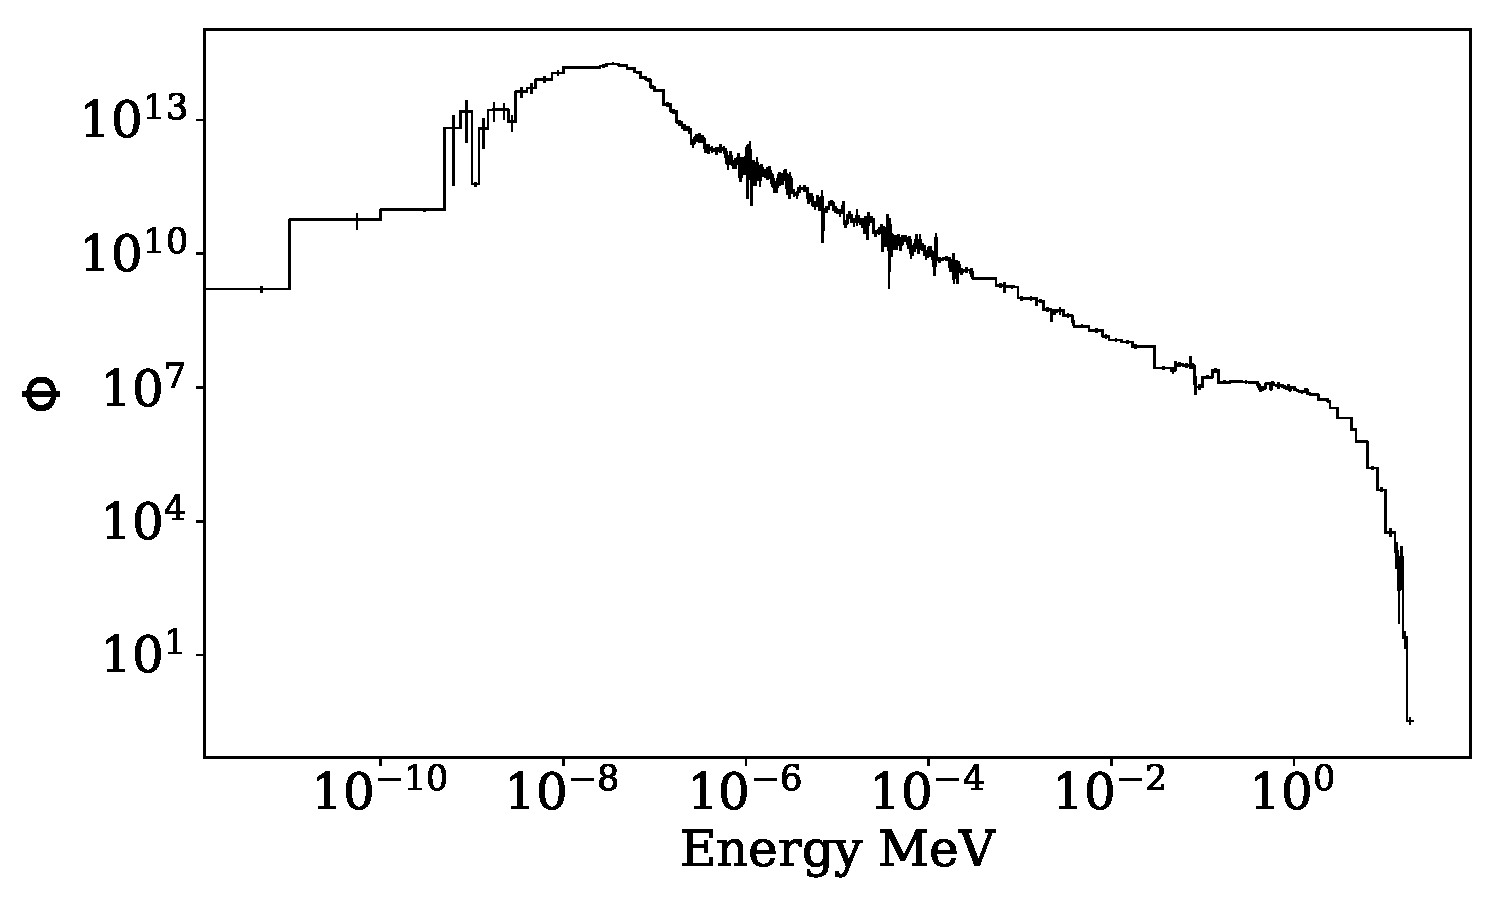
\includegraphics[height=4in]{tex/figures/flux_erg.pdf}
\caption[Flux vs. Energy]{The differential flux as a function of energy.}
\label{fig:flux_erg}
\end{figure}

% this is the differential flux as a function of energy
Shown in \FIG{fig:flux_erg} is the differential flux as a function of energy.
% it has been integrated over both angle and tally region
This has been integrated over both angle as well as the seven tally regions.
% because of this, the spectrum resembles that which one would find within the core
The spectrum resembles that which one would find within a reactor core.
% you've got your watt distribution % you've got your 1/E region % you've got your maxwellian distrubution
Centered around 1 MeV is the Watt fission distribution, the intermediate region is comprised of $1/E$ slowing down neutrons, and peaking around $3 \times 10^{-8}$ MeV is the Maxwellian distribution.
% the main contribution to this tally is line of sight down the beam
This is likely because the line-of-sight neutrons streaming from the core are the primary component to this flux tally.
% as you can see, those are clearly on display because, ya know it should look like that
The borated polyethylene within the collimator is a very strong absorber and also very long, so it is unlikely that moderated neutrons escape and manage to contribute to the tally.

% there are two noisy locations
There are also two regions seen in this plot that are heavily affected by statistical noise, the slower half of the $1/E$ region and the slow tail of the Maxwellian distribution.
% this is because of low probability tallies
This is because there is such a low probability that a neutron at that energy will be tallied.
% this is because of small bin widths in the 1/e region and low probability within the super slow region
Specifically, within the scale252 bin structure, there are several narrow bins within the $1/E$ region, and tally probability is proportional to the bin width times the true flux, therefore, it is reasonable to see high errors within that region.
The flux in the tail end of the Maxwellian distribution is also very low, causing the poor resolution within that region.
These could ultimately be resolved via simulation of more particles.


%\clearpage

%
\begin{figure}[htb]
\centering
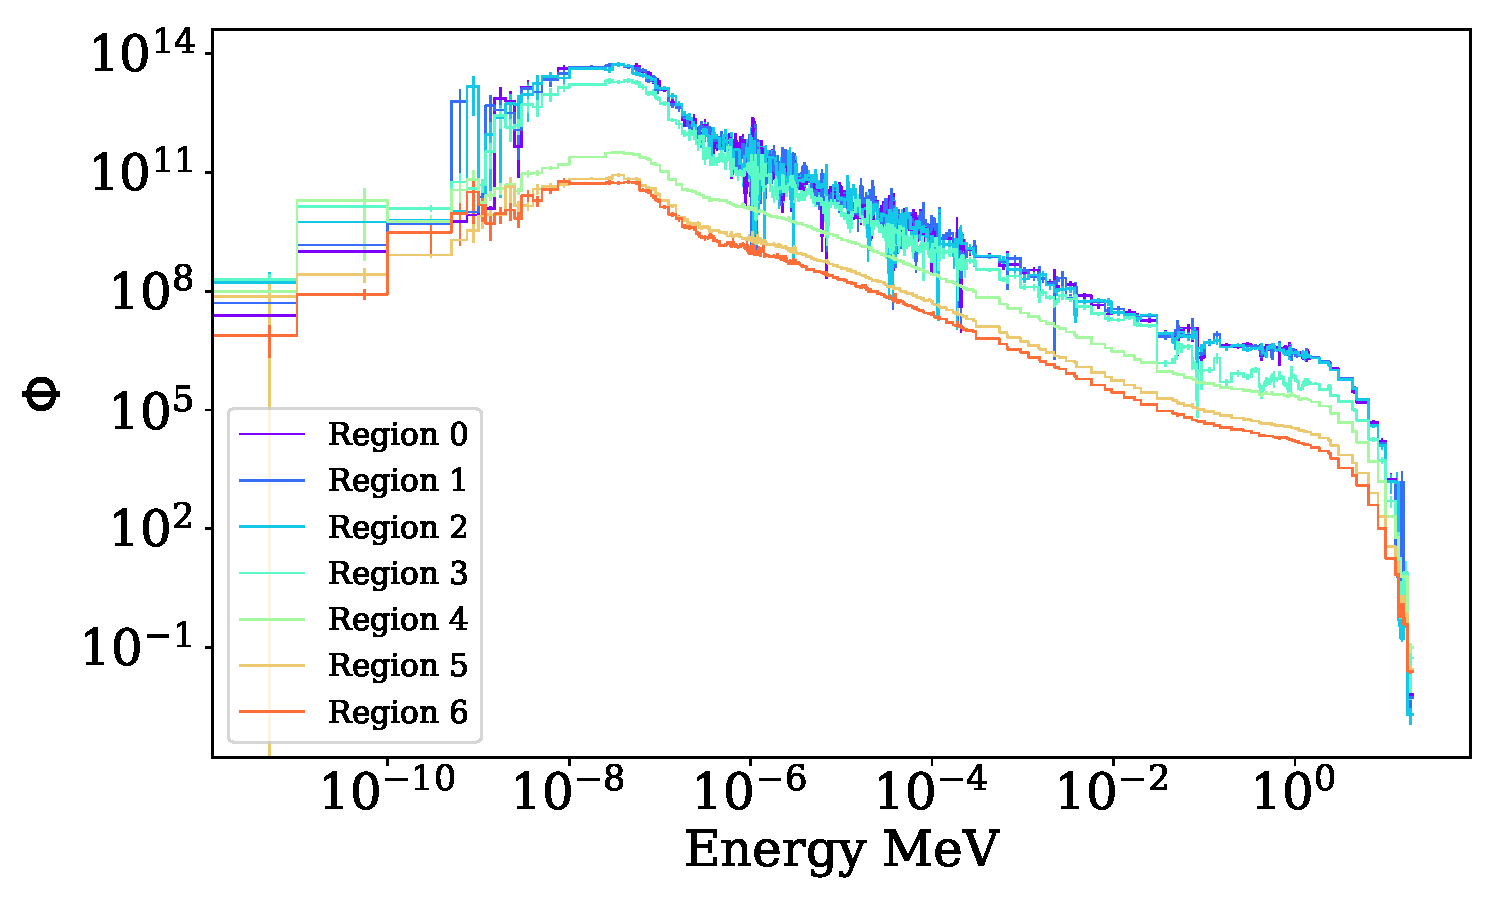
\includegraphics[height=4in]{tex/figures/flux_rad_erg.pdf}
\caption[Regional Flux vs. Energy]{The differential flux plotted against energy and broken into each tally region.}
\label{fig:flux_rad_erg}
\end{figure}

% the erg dependent flux can be seen broken down into region in figure whatever.
The energy-dependent flux can be seen broken down into its separate regional tallies within \FIG{fig:flux_rad_erg}.
% regions 0-7 refer to whatever
Recall, regions 0-2 are equal-area tallies within the beam, region 3 refers to the aluminum collimator, and regions 5-7 are equal-area tallies within the borated polyethylene.
% this gives us a first glance at comparing magnitudes
This plot gives us a first glance at comparing the magnitudes within each region.
Over three orders of magnitude lie between the highest and lowest regional fluxes.
% let's comment on noise for a sec, too
The noise problem \FIG{fig:flux_erg} is also amplified here, as separating the tallies by region furthur slows individual tally bin convergence.
However, it is still possible to draw meaningful conclusions from this plot.
% okay, first, there's like no difference in the first three
First, apart from statistical noise, there is no obvious difference between the spectra within the in-beam regions.
% in the aluminum, the fast flux seems flattened
It is in the aluminum where the flux begins to deviate, being separated both by magnitude and also exibiting a flatness within the fast region.
% the bp sections are clearly moderated
Differences seen in the borated polyethylene regions are much more obvious, as the spectra are clearly moderated variants of those in-beam.
% look how the fast peak shrinks the further out you go
The farthur from the center of the beam, the more flat the fast region becomes.
% the 1/e region shows some curvature here. interesting
The $1/E$ region begins to demonstrate some curvature, which is likely in relation to the absorption and scattering cross sections of the borated polyethylene.
% also, maxwell is flattened
The Maxwellian distributions within these sections are also flattened and exibit much less drastic tapering in the slowest regions.

%\clearpage

%
\begin{figure}[htb]
\centering
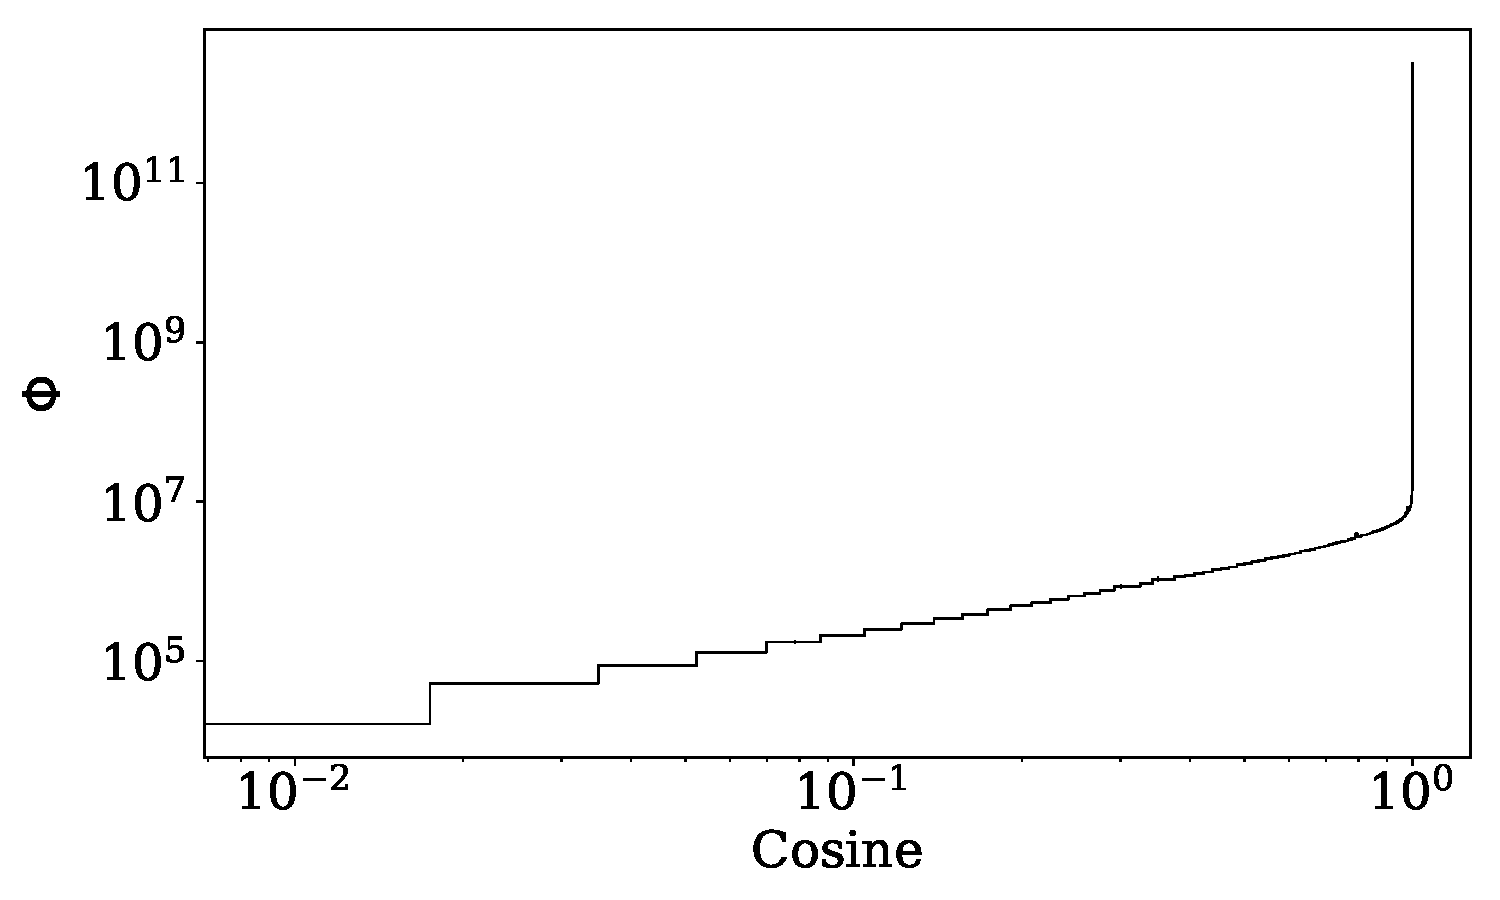
\includegraphics[height=4in]{tex/figures/flux_cos.pdf}
\caption[Flux vs. Angle]{The energy-integrated flux as a fuction of angle.}
\label{fig:flux_cos}
\end{figure}

% this is the figure showing the flux as a function of angle from
The flux as a function of angle can be seen in \FIG{fig:flux_cos}.
% right away, it's apparent that the collimator is doing its job
Right away, it is apparent that the collimator is effectively constricting the neutron beam.
% these fluxes span N orders of magnitude across the way
The fluxes in the plot span over eight orders of magnitude.
% the sharp increase at the right is caused by the line-of-sight through the beam
This incredibly sharp upturn at the right is due to the line-of-sight neutrons again being the largest contributor to the flux.
% outside of that, there's just a gradual exponential decrease as you go off beam through the BP region
Outside of that, the rest of this flux is goverened by a smooth exponential tapering caused by scattering within the collimator.

%\clearpage

%
\begin{figure}[htb]
\centering
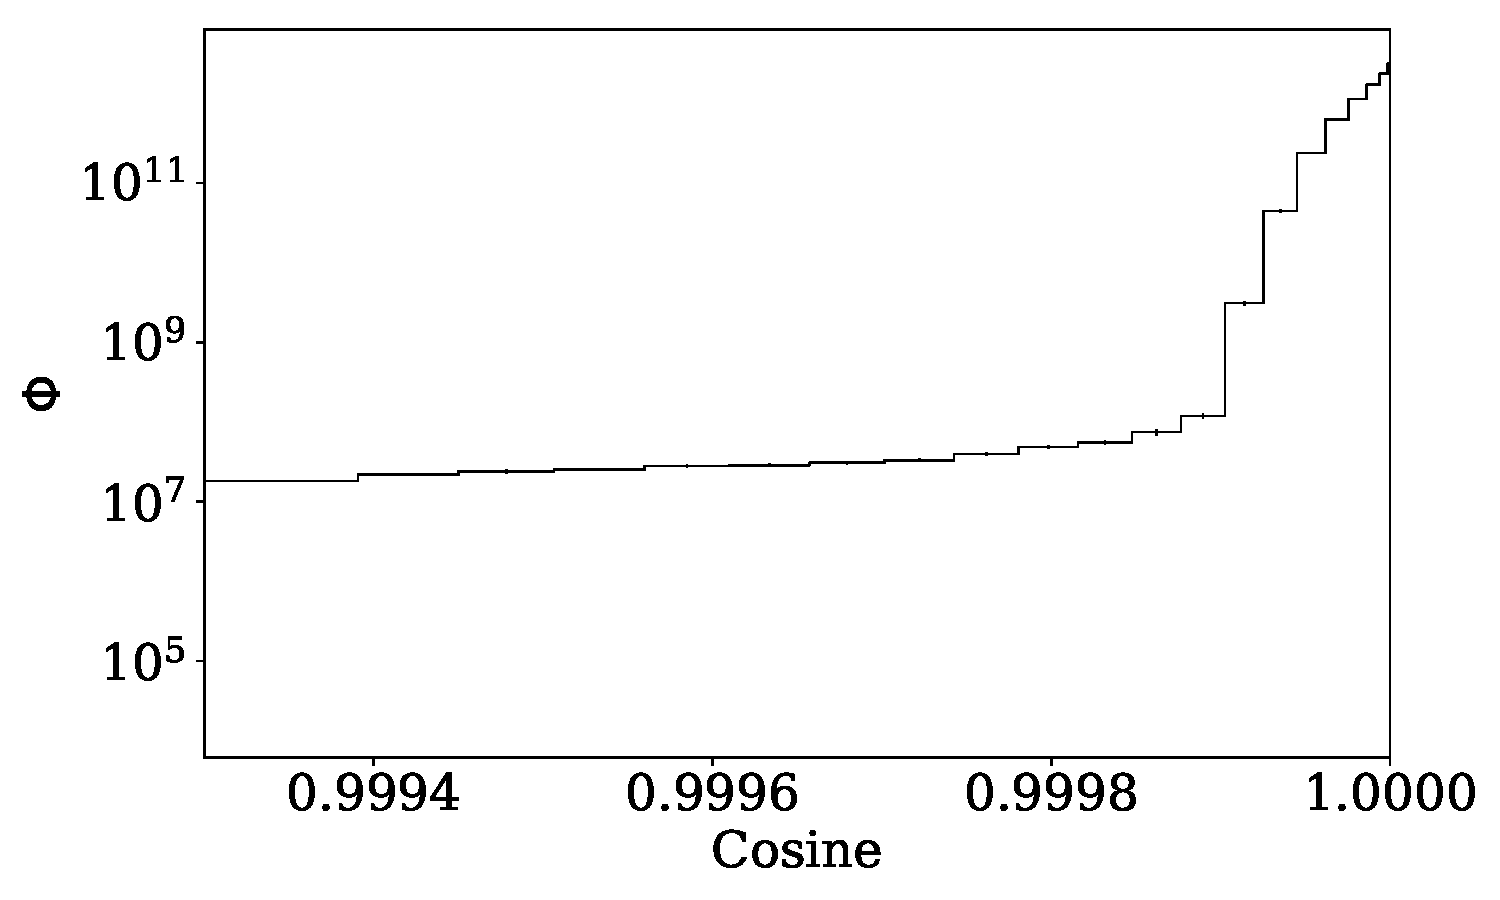
\includegraphics[height=4in]{tex/figures/flux_cos_detail.pdf}
\caption[Detailed Flux vs. Angle]{A detailed view of the NEBP angular flux.}
\label{fig:flux_cos_detail}
\end{figure}

% this is a closer look a the peak angular flux
Seen in \FIG{fig:flux_cos_detail} is a closer look at the forward peak in the angular flux.
% within a cosine of 0.9999 and 1.0000 there's a jump of over 5 orders of magnitude.
Within cosine values of 0.9999 and 1.0000 a jump of over five orders of magnitude occurs.
% this allows us to comment on the relationship between scattering and absorption within the collimator
This allows us to comment on the relationship between scattering and absorption within the collimator.
% bounds on the sharpness of the peak matches the maximum angle that a neutron can travel within the collimator without an interaction.
The bounds on the sharpness of the peak match the maximum line-of-sight angle within the aluminum tube in the beam.
The neutrons within this peak are managing to stream down the collimator from the core without interacting on the way.
% if scattering was dominant within the collimator, this peak would appear much flatter, but since it's not, the boron within the collimator is likely the reason.
This suggests that absorption dominates interactions within the collimator.
If scattering was more likely, this peak would be much smoother, but, instead, the neutrons entering the collimator are being removed.

%\clearpage

% the radial flux broken into tally regions
\begin{figure}[htb]
\centering
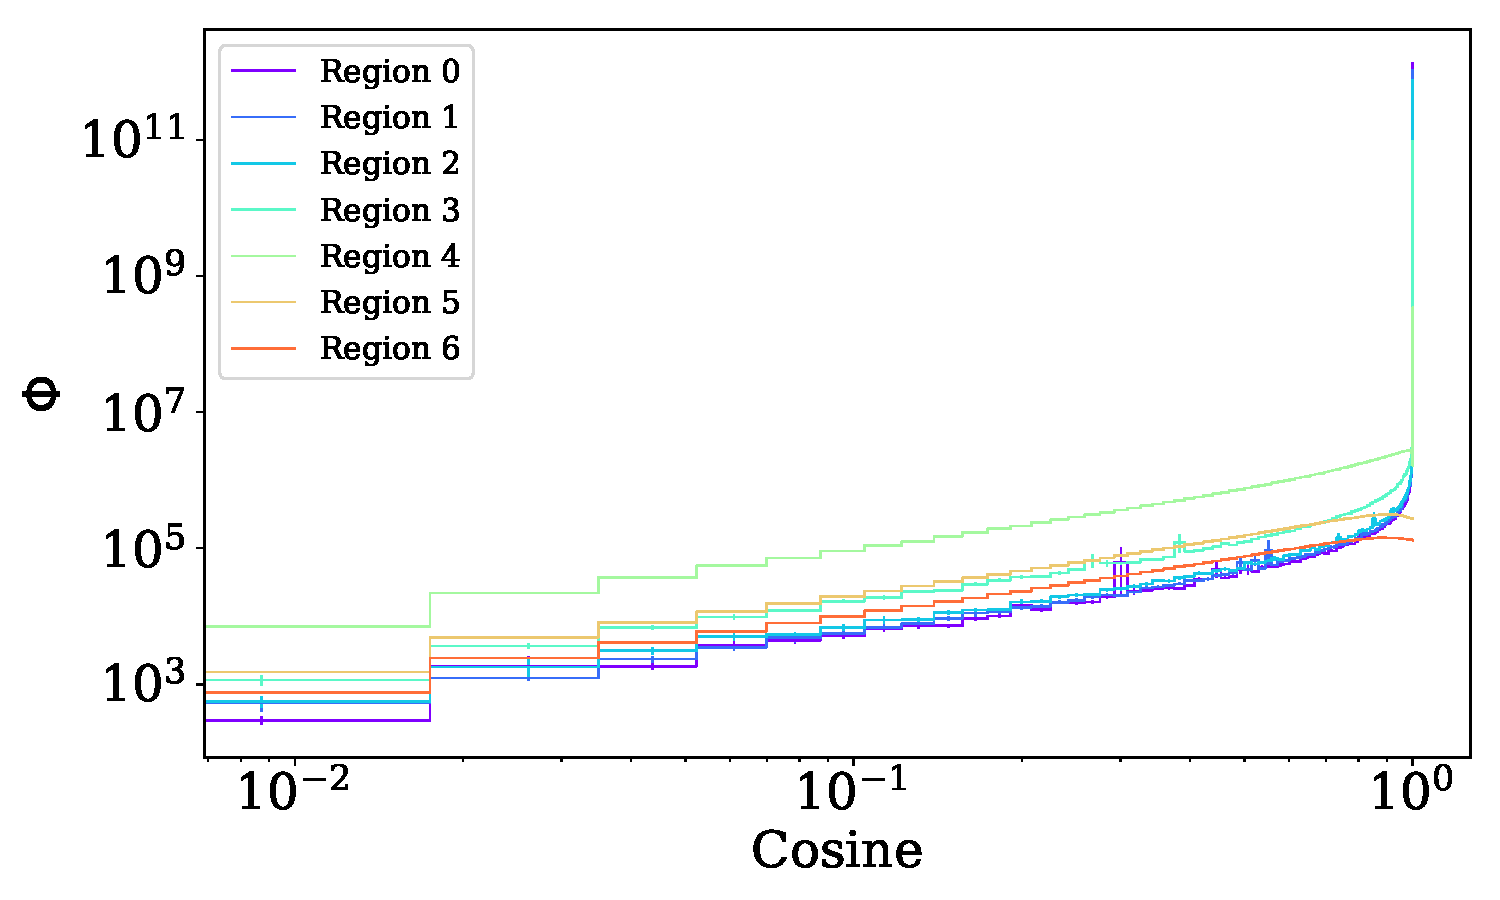
\includegraphics[height=4in]{tex/figures/flux_rad_cos.pdf}
\caption[Regional Flux vs. Angle]{The NEBP radial flux broken into tally regions.}
\label{fig:flux_rad_cos}
\end{figure}

% regional angular flux shown here
Here, in \FIG{fig:flux_rad_cos} is the anglur flux broken into tally regions.
% similar to energy dependent flux, there's little deviation that can be seen between regions 0-2, except there's question about the magnitude here
Similar to the energy dependent flux plotted above, there is little deviation that can be seen between regions 0-2, although there is slight differences in the magnitudes.
% definite jump in the aluminum section
The aluminum section, section 3, exhibits much more isotropy, as the flux seen on this plot appears much higher than the others, it is the first non-void material encountered by the neutrons.
% the anisotropy is much higher within the outer regions
This anisotropy is still much higher in the borated polyethylene sections.
% they are still forward peaked, though, but that doesn't happen cos=1.000 but rather at an angle.
Each region has a peak located close to 1.000; however, it is not always the highest at 1.000.
This is likely due to the single or double scatterings that have to happen near the end of the beam to move a neutron to those regions.

%\clearpage

% detailed view of the regional flux vs angle
\begin{figure}[htb]
\centering
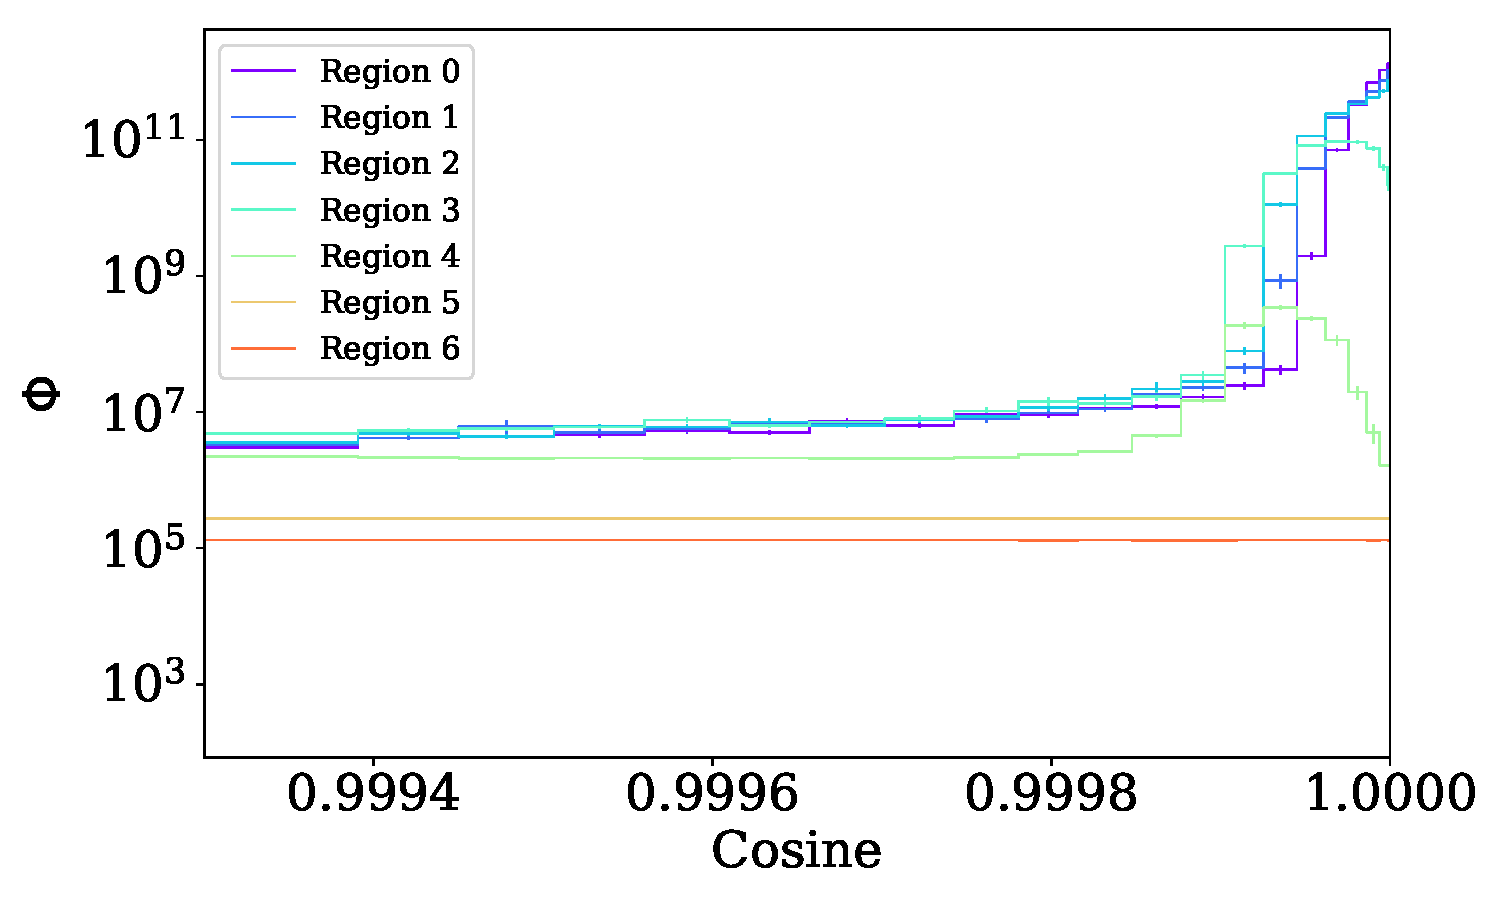
\includegraphics[height=4in]{tex/figures/flux_rad_cos_detail.pdf}
\caption[Detailed Regional Flux vs. Angle]{A detailed view of the angular flux broken into tally regions.}
\label{fig:flux_rad_cos_detail}
\end{figure}

% data shown in figure is a detailed view of the plot on the previous page
In \FIG{fig:flux_rad_cos_detail} is the detailed view of the data from \FIG{fig:flux_rad_cos}.
% this shows in greater detail the specifics of the forward peaking that happends in the angular flux
This shows greater detail on the peak specifics of the angular fluxes.
% regions 0-2 all have the highest bin being the most forward, however the distribution broadens as you move outward
The in-beam regions are all forward peaked, with the highest bin being at cos = 1.000; however, the distribution tends to broaden when moving outward.
% this trend is even true in the aluminum
This trend continues in the aluminum section.
% in the BP in region 4, the peak lies slightly off center, likely related to scattering behavior that allowed neutrons to get to that tally
In region 4 in the borated polyethylene, this peak appears slightly off axis, which is related to the scattering or ``edge-clipping'' effects that would transport a neutron to that region.
% in this view, regions 5 and 6 appear isotropic, likely because a neutron to encounter one of those tally planes would have scattered several times
In this view, regions 5 and 6 appear isotropic, likely because any neutron to encounter either of those tally planes would have scattered several times, effectively diffusing the spectrum.

%\clearpage

% the flux as a function of tally region
\begin{figure}[htb]
\centering
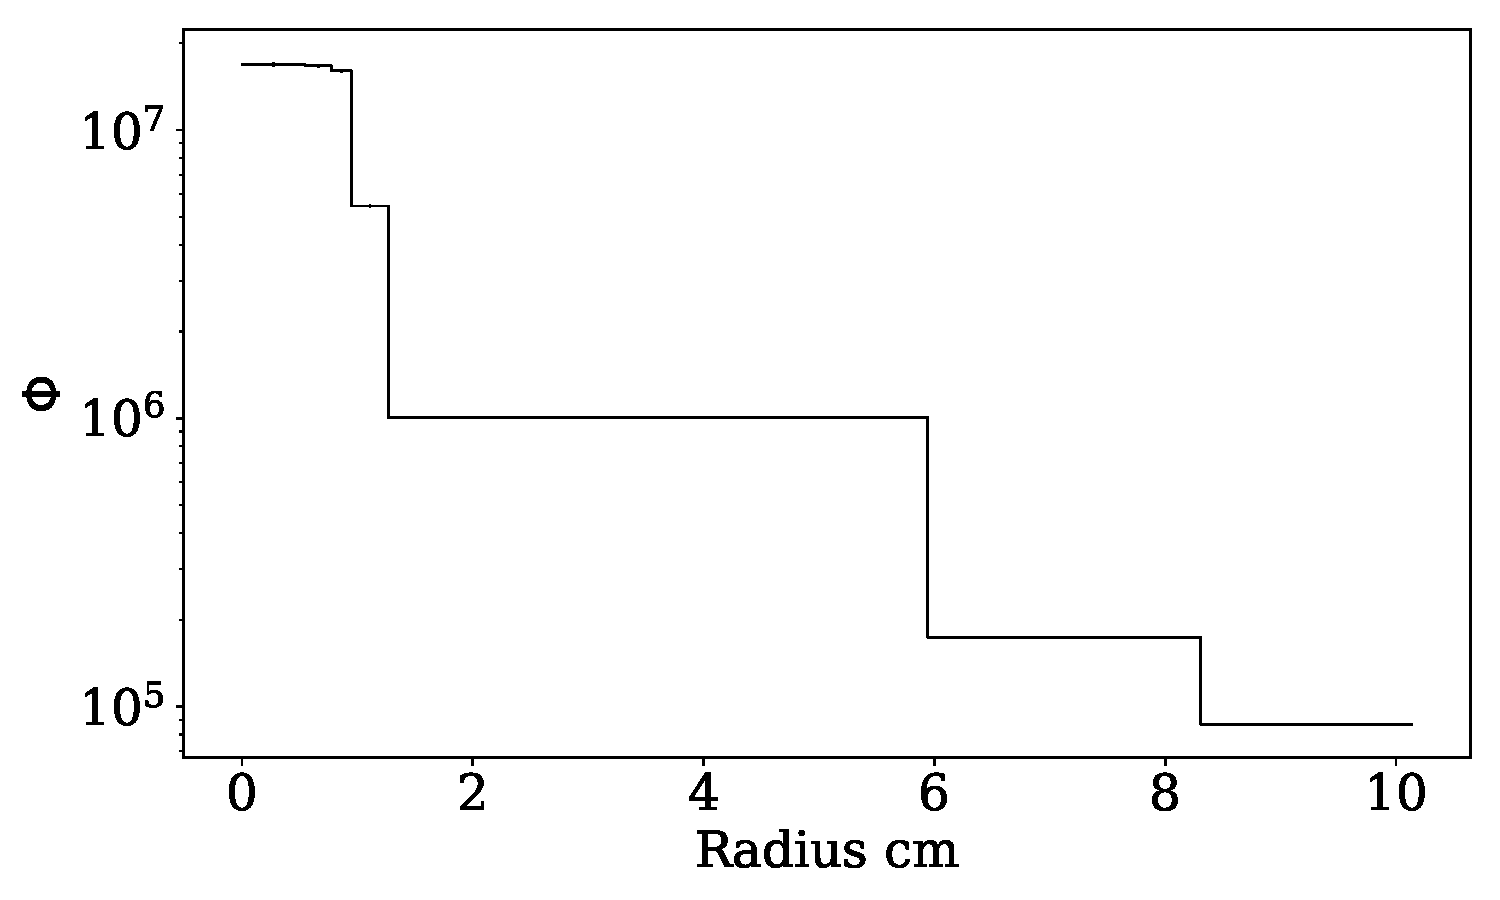
\includegraphics[height=4in]{tex/figures/flux_rad.pdf}
\caption[Regional Flux]{The NEBP flux as a function of tally region.}
\label{fig:flux_rad}
\end{figure}

% here, finally, we can see a direct comparison of the fluxes within each region of the tally
Here, finally, we can see a direct comparison of the fluxes within each tally region in \FIG{fig:flux_rad}.
% there is very little difference between the tallies within the beam port
There is very little difference between the magnitude of the tallies in the beam.
% then, from each region in the collimator, we see a tapering that leads to a two order of magnitude difference in the flux from the innermost to outermost region
Then, moving outward through each region in the collimator, we see a tapering that leads to a difference of two orders of magnitude in the flux from the innermost to the outermost region.


%\clearpage
